\documentclass[aspectratio=169,10pt]{beamer}
\usepackage[T1]{fontenc}
\usepackage{amsmath,amssymb,amsfonts}
\usepackage{bm}
\usepackage{tikz}
\usepackage{xcolor}
\usetikzlibrary{arrows.meta,positioning,shapes,calc}

\definecolor{parchment}{HTML}{F4E8C8}
\definecolor{paper}{HTML}{FAF1D8}
\definecolor{ink}{HTML}{1A1A1A}
\definecolor{inkgray}{HTML}{5A5A5A}
\definecolor{accentred}{HTML}{8B1A1A}
\definecolor{accentgreen}{HTML}{2D5F2C}
\definecolor{accentblue}{HTML}{1F4E79}
\definecolor{redbg}{HTML}{F7E0DE}
\definecolor{grnbg}{HTML}{E0EBDC}
\definecolor{blubg}{HTML}{DDE6EF}
\definecolor{labelbg}{HTML}{EFE0B0}

\usefonttheme{serif}
\setbeamercolor{background canvas}{bg=parchment}
\setbeamercolor{normal text}{fg=ink}
\setbeamercolor{structure}{fg=ink}
\setbeamercolor{frametitle}{fg=ink,bg=parchment}
\setbeamercolor{title}{fg=ink}
\setbeamercolor{itemize item}{fg=ink}
\setbeamercolor{itemize subitem}{fg=ink}
\setbeamercolor{item}{fg=ink}
\setbeamercolor{caption name}{fg=ink}
\setbeamertemplate{navigation symbols}{}
\setbeamertemplate{itemize item}{\textbullet}

\setbeamertemplate{frametitle}{%
  \vspace{0.30em}%
  \begin{center}%
    {\bfseries\Large\insertframetitle\par}%
    \vspace{0.28em}%
    {\color{ink}\rule{0.86\paperwidth}{0.4pt}}%
  \end{center}%
  \vspace{0.10em}%
}
\setbeamertemplate{footline}{%
  \hbox to \paperwidth{\hfil\itshape\small\insertframenumber\hspace{0.7em}}%
  \vspace{0.35em}%
}

\newcommand{\vY}{\bm{Y}}
\newcommand{\vy}{\bm{y}}
\newcommand{\vA}{\bm{A}}
\newcommand{\vB}{\bm{B}}
\newcommand{\valpha}{\bm{\alpha}}
\newcommand{\vn}{\bm{n}}
\newcommand{\vs}{\bm{s}}
\newcommand{\vW}{\bm{W}}
\newcommand{\T}{^{\mathsf T}}
\newcommand{\Hh}{^{\mathsf H}}
\newcommand{\norm}[1]{\left\lVert #1\right\rVert}
\DeclareMathOperator*{\argmin}{arg\,min}

\tikzset{
  flowbox/.style={draw=ink,fill=paper,line width=0.6pt,
                  minimum width=2.5cm,minimum height=1.0cm,
                  align=center,font=\small\bfseries,inner sep=4pt},
  smallbox/.style={draw=ink,fill=paper,line width=0.4pt,
                   minimum width=0.7cm,minimum height=0.55cm,
                   inner sep=2pt,align=center,font=\footnotesize\itshape},
  method/.style={draw=accentgreen,fill=grnbg,line width=1.0pt,
                 align=center,font=\small\bfseries,inner sep=6pt},
  issue/.style={draw=accentred,fill=redbg,line width=1.0pt,
                align=center,font=\small\bfseries,inner sep=6pt},
  idea/.style={draw=accentblue,fill=blubg,line width=1.0pt,
               align=center,font=\small\bfseries,inner sep=6pt},
  flowarr/.style={-{Stealth[length=2.5mm,width=2mm]},line width=0.7pt},
  softarr/.style={-{Stealth[length=2mm,width=1.6mm]},line width=0.5pt,color=inkgray}
}

\newcommand{\bottomnote}[1]{%
  \begin{center}{\itshape\small #1}\end{center}}

\newcommand{\papercover}[4]{%
  \begin{frame}[plain]
    \vfill
    \begin{center}
      {\bfseries\Huge #1\par}
      \vspace{0.8cm}
      {\Large #2\par}
      \vspace{0.35cm}
      {\itshape\large\color{inkgray}#3\par}
      \vspace{0.55cm}
      {\small\texttt{\detokenize{#4}}\par}
    \end{center}
    \vfill
  \end{frame}}

\newcommand{\twocolmodel}[4]{%
  \begin{columns}[T,onlytextwidth]
    \begin{column}{0.48\textwidth}#1\end{column}
    \begin{column}{0.48\textwidth}#2\end{column}
  \end{columns}
  \bottomnote{#3\\#4}}


\usetikzlibrary{decorations.pathreplacing,decorations.pathmorphing,shapes.misc}

\newcommand{\jj}{\mathrm{j}}
\newcommand{\sinc}{\operatorname{sinc}}
\newcommand{\rx}{\mathrm{rx}}
\newcommand{\tx}{\mathrm{tx}}
\newcommand{\diag}{\mathrm{diag}}

% ===== visual helpers used only in this deck =====
\tikzset{
  stepbadge/.style={
    draw=ink, fill=labelbg, line width=0.6pt, circle,
    inner sep=0pt, minimum size=0.85cm,
    font=\bfseries\small
  },
  notecard/.style={
    draw=ink, fill=paper, line width=0.5pt, rounded corners=2pt,
    align=center, inner sep=5pt, font=\small
  },
  greencard/.style={
    draw=accentgreen, fill=grnbg, line width=0.8pt, rounded corners=2pt,
    align=center, inner sep=5pt, font=\small
  },
  redcard/.style={
    draw=accentred, fill=redbg, line width=0.8pt, rounded corners=2pt,
    align=center, inner sep=5pt, font=\small
  },
  bluecard/.style={
    draw=accentblue, fill=blubg, line width=0.8pt, rounded corners=2pt,
    align=center, inner sep=5pt, font=\small
  },
  thinkbubble/.style={
    draw=accentblue, fill=blubg!75, line width=0.6pt,
    rounded corners=6pt, align=center, inner sep=6pt,
    font=\itshape\small
  },
  brace/.style={decorate, decoration={brace, amplitude=4pt, raise=2pt}, line width=0.55pt, color=inkgray}
}

% Step badge sits BELOW the title rule (the rule is around 1.4cm from page top
% in this 16:9 deck). 0.62cm badge + a one-line caption to the right.
\newcommand{\stepbadgehdr}[2]{%
  \begin{tikzpicture}[remember picture,overlay]
    \node[stepbadge,anchor=north west,minimum size=0.62cm,font=\bfseries\footnotesize]
      at ([xshift=0.30cm,yshift=-1.62cm]current page.north west) {#1};
    \node[anchor=west,font=\scriptsize\itshape\color{inkgray}]
      at ([xshift=1.00cm,yshift=-1.92cm]current page.north west) {#2};
  \end{tikzpicture}%
}

% Stage-4 substage breadcrumb (top-right). Used by frames 4a..4f.
% #1 = active index 1..6, #2 = caption next to badge "4"
\newcommand{\substagepill}[3]{%
  % #1 active index, #2 this pill's index, #3 this pill's label
  \ifnum#2=#1
    \node[fill=accentgreen,draw=accentgreen,line width=0.5pt,
          rounded corners=2pt,inner sep=2pt,
          minimum width=0.62cm,minimum height=0.36cm,
          font=\bfseries\tiny\color{paper}] {#3}%
  \else
    \node[fill=paper,draw=inkgray!50,line width=0.4pt,
          rounded corners=2pt,inner sep=2pt,
          minimum width=0.62cm,minimum height=0.36cm,
          font=\bfseries\tiny\color{inkgray}] {#3}%
  \fi
}
\newcommand{\stagefourhdr}[2]{%
  \begin{tikzpicture}[remember picture,overlay]
    % left: the stage badge + caption (same as \stepbadgehdr)
    \node[stepbadge,anchor=north west,minimum size=0.62cm,font=\bfseries\footnotesize]
      at ([xshift=0.30cm,yshift=-1.62cm]current page.north west) {4};
    \node[anchor=west,font=\scriptsize\itshape\color{inkgray}]
      at ([xshift=1.00cm,yshift=-1.92cm]current page.north west) {#2};
    % right: 6-pill breadcrumb (a row of pills with thin connectors)
    \node[anchor=north east] at ([xshift=-0.30cm,yshift=-1.50cm]current page.north east) {%
      \begin{tikzpicture}[x=0.78cm,y=0.5cm]
        \foreach \i in {1,2,3,4,5} {
          \draw[inkgray!50,line width=0.4pt] ({(\i-1)+0.32},0) -- ({\i-0.32},0);
        }
        \begin{scope}[shift={(0,0)}] \substagepill{#1}{1}{4a}; \end{scope}
        \begin{scope}[shift={(1,0)}] \substagepill{#1}{2}{4b}; \end{scope}
        \begin{scope}[shift={(2,0)}] \substagepill{#1}{3}{4c}; \end{scope}
        \begin{scope}[shift={(3,0)}] \substagepill{#1}{4}{4d}; \end{scope}
        \begin{scope}[shift={(4,0)}] \substagepill{#1}{5}{4e}; \end{scope}
        \begin{scope}[shift={(5,0)}] \substagepill{#1}{6}{4f}; \end{scope}
      \end{tikzpicture}%
    };
  \end{tikzpicture}%
}
% Backward-compat alias (no leading-digit issue this way)
\let\stagefourhdrA\stagefourhdr

\begin{document}

% =====================================================================
% Cover
% =====================================================================
\begin{frame}[plain]
  \vspace{0.6cm}
  \begin{center}
    {\bfseries\Huge Doppler, ICI \& Partial FFT\par}
    \vspace{0.20cm}
    {\Large\itshape ICI as an unfinished de-spinning loop\par}

    \vspace{0.55cm}
    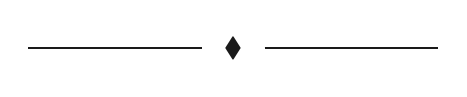
\begin{tikzpicture}
      \draw[ink,line width=0.5pt] (-2.6,0) -- (-0.4,0);
      \node at (0,0) {\color{ink}$\blacklozenge$};
      \draw[ink,line width=0.5pt] (0.4,0) -- (2.6,0);
    \end{tikzpicture}
    \vspace{0.45cm}

    % Hero illustration: clean carrier comb -> Doppler skew -> partial-FFT recovery
    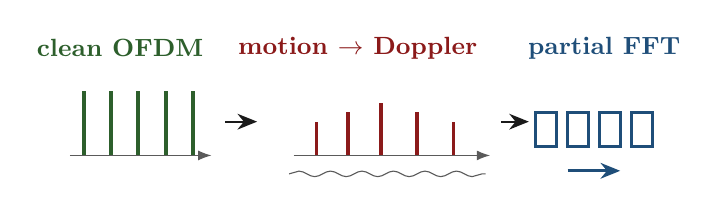
\begin{tikzpicture}[x=0.58cm,y=0.78cm,>=Latex]
      % left: clean comb
      \node[font=\small\bfseries\color{accentgreen}] at (-5.4,1.55) {clean OFDM};
      \foreach \x in {-6.2,-5.6,-5.0,-4.4,-3.8} {
        \draw[accentgreen,line width=1.4pt] (\x,-0.2) -- (\x,0.85);
      }
      \draw[inkgray,->] (-6.5,-0.2) -- (-3.4,-0.2);

      \node[font=\small\bfseries\color{accentred}] at (-0.2,1.55) {motion $\to$ Doppler};
      \foreach \x/\h in {-1.10/0.55,-0.42/0.70,0.32/0.85,1.10/0.70,1.90/0.55} {
        \draw[accentred,line width=1.4pt] (\x,-0.2) -- (\x,{-0.2+\h});
      }
      % "wind" wiggle behind
      \draw[inkgray,decorate,decoration={snake,amplitude=1.0pt,segment length=4mm}]
        (-1.7,-0.5) -- (2.6,-0.5);
      \draw[inkgray,->] (-1.6,-0.2) -- (2.7,-0.2);

      \node[font=\small\bfseries\color{accentblue}] at (5.2,1.55) {partial FFT};
      % four short windows -> one big arrow
      \foreach \x in {3.7,4.4,5.1,5.8} {
        \draw[accentblue,line width=1.0pt] (\x,-0.05) rectangle ++(0.45,0.55);
      }
      \draw[flowarr,color=accentblue,line width=1.0pt] (4.4,-0.45) -- (5.55,-0.45);

      % connecting arrows
      \draw[flowarr,color=ink] (-3.10,0.35) -- (-2.40,0.35);
      \draw[flowarr,color=ink] (2.95,0.35) -- (3.55,0.35);
    \end{tikzpicture}

    \vspace{0.65cm}
    {\itshape\small\color{inkgray}A companion to the OFDM Doppler workbench and the JUNA/RPC talk\par}
  \end{center}
\end{frame}

% =====================================================================
% Roadmap
% =====================================================================
\begin{frame}{Where this tutorial is going}
\small
\begin{center}
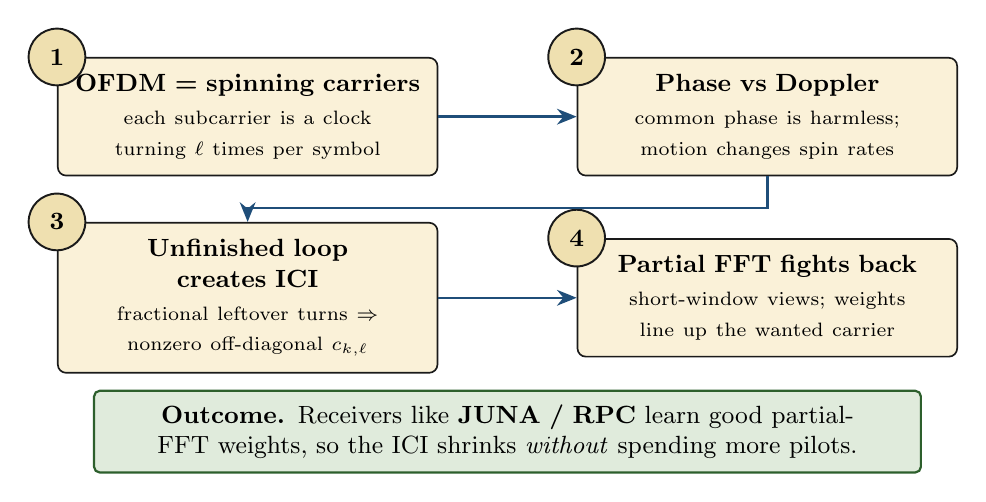
\begin{tikzpicture}[x=1.0cm,y=1.0cm,>=Latex,
   roadcard/.style={draw=ink, fill=paper, line width=0.6pt,
                    rounded corners=3pt, align=center, inner sep=6pt,
                    text width=4.4cm, minimum height=1.35cm, font=\small},
   roadbadge/.style={circle, draw=ink, fill=labelbg, line width=0.7pt,
                     minimum size=0.72cm, inner sep=0pt, font=\bfseries\small}]

  % Top row
  \node[roadcard] (s1) at (-3.3,1.3) {%
    \textbf{OFDM = spinning carriers}\\[0.10em]
    \scriptsize each subcarrier is a clock turning $\ell$ times per symbol};
  \node[roadcard] (s2) at (3.3,1.3) {%
    \textbf{Phase vs Doppler}\\[0.10em]
    \scriptsize common phase is harmless; motion changes spin rates};

  % Bottom row
  \node[roadcard] (s3) at (-3.3,-1.0) {%
    \textbf{Unfinished loop creates ICI}\\[0.10em]
    \scriptsize fractional leftover turns $\Rightarrow$ nonzero off-diagonal $c_{k,\ell}$};
  \node[roadcard] (s4) at (3.3,-1.0) {%
    \textbf{Partial FFT fights back}\\[0.10em]
    \scriptsize short-window views; weights line up the wanted carrier};

  % Step badges on top-left corner of each card (outside the card box)
  \node[roadbadge] at (s1.north west) {1};
  \node[roadbadge] at (s2.north west) {2};
  \node[roadbadge] at (s3.north west) {3};
  \node[roadbadge] at (s4.north west) {4};

  % Curved soft arrows
  \draw[flowarr,color=accentblue,line width=0.9pt] (s1.east) -- (s2.west);
  \draw[flowarr,color=accentblue,line width=0.9pt] (s2.south) -- ($(s2.south) + (0,-0.4)$) -| (s3.north);
  \draw[flowarr,color=accentblue,line width=0.9pt] (s3.east) -- (s4.west);

  % Outcome banner
  \node[greencard,minimum width=10.5cm,text width=10.0cm,font=\small]
    at (0,-2.7) {%
    \textbf{Outcome.} Receivers like \textbf{JUNA / RPC} learn good partial-FFT weights, so the ICI shrinks \emph{without} spending more pilots.};
\end{tikzpicture}
\end{center}

\vspace{-0.10cm}
\begin{center}\footnotesize
  Each step is \emph{picture first, formula second}.\quad
  \textcolor{accentgreen}{\textbf{green}}=wanted,\quad
  \textcolor{accentred}{\textbf{red}}=leakage,\quad
  \textcolor{accentblue}{\textbf{blue}}=receiver tool.
\end{center}
\end{frame}

% =====================================================================
% 1a. Full OFDM chain
% =====================================================================
\begin{frame}{1a. Full OFDM chain: where the loop lives}
\stepbadgehdr{1}{modulate, transmit, de-spin, then decide bits}
\small
\begin{center}
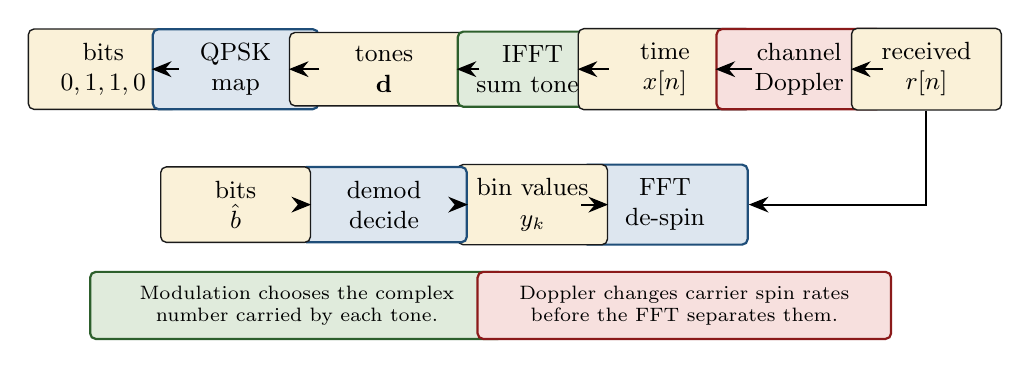
\begin{tikzpicture}[x=0.82cm,y=0.80cm,>=Latex]
  \node[notecard,text width=1.55cm] (bits) at (-6.2,1.0) {bits\\$0,1,1,0$};
  \node[bluecard,text width=1.75cm] (mod) at (-4.15,1.0) {QPSK\\map};
  \node[notecard,text width=2.05cm] (tones) at (-1.85,1.0) {tones\\$\mathbf d$};
  \node[greencard,text width=1.55cm] (ifft) at (0.45,1.0) {IFFT\\sum tones};
  \node[notecard,text width=1.85cm] (x) at (2.50,1.0) {time\\$x[n]$};
  \node[redcard,text width=1.75cm] (chan) at (4.58,1.0) {channel\\Doppler};
  \node[notecard,text width=1.55cm] (r) at (6.55,1.0) {received\\$r[n]$};

  \node[bluecard,text width=1.75cm] (fft) at (2.50,-1.15) {FFT\\de-spin};
  \node[notecard,text width=1.55cm] (yk) at (0.45,-1.15) {bin values\\$y_k$};
  \node[bluecard,text width=1.75cm] (dem) at (-1.85,-1.15) {demod\\decide};
  \node[notecard,text width=1.55cm] (bhat) at (-4.15,-1.15) {bits\\$\hat b$};

  \draw[flowarr] (bits) -- (mod);
  \draw[flowarr] (mod) -- (tones);
  \draw[flowarr] (tones) -- (ifft);
  \draw[flowarr] (ifft) -- (x);
  \draw[flowarr] (x) -- (chan);
  \draw[flowarr] (chan) -- (r);
  \draw[flowarr] (r.south) |- (fft.east);
  \draw[flowarr] (fft) -- (yk);
  \draw[flowarr] (yk) -- (dem);
  \draw[flowarr] (dem) -- (bhat);

  \node[greencard,text width=4.9cm,font=\scriptsize] at (-3.20,-2.75)
    {Modulation chooses the complex number carried by each tone.};
  \node[redcard,text width=4.9cm,font=\scriptsize] at (2.80,-2.75)
    {Doppler changes carrier spin rates before the FFT separates them.};
\end{tikzpicture}
\end{center}
\bottomnote{The loop picture lives inside the FFT block: an FFT bin de-spins one carrier and averages the result.}
\end{frame}

% =====================================================================
% 1b. What is OFDM (intuition)
% =====================================================================
\begin{frame}{1b. OFDM in one picture}
\stepbadgehdr{1}{the receiver-side intuition we are building toward}
\small
\begin{columns}[T,onlytextwidth]
  \begin{column}{0.42\textwidth}
    \vspace{0.2cm}
    \begin{itemize}\setlength{\itemsep}{0.40em}
      \item OFDM splits a bit stream onto \emph{many narrow carriers}, all sent at the same time.
      \item Carrier $\ell$ is a sine wave with frequency $\ell$ (in units of $1/T$, one OFDM symbol).
      \item During one symbol of length $T$, carrier $\ell$ completes \textbf{exactly $\ell$ full turns}.
      \item All carriers add up to a single waveform $s(t)$, which the transmitter sends.
    \end{itemize}
  \end{column}
  \begin{column}{0.55\textwidth}
    \begin{center}
    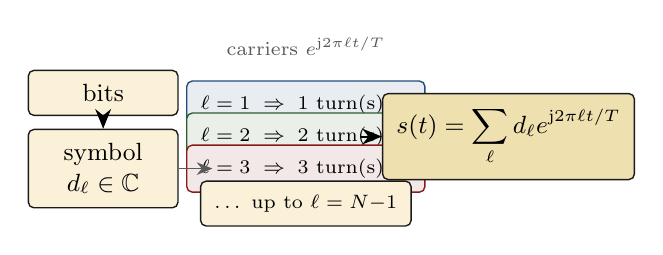
\begin{tikzpicture}[x=0.78cm,y=0.74cm,>=Latex]
      % left column: bits and symbols
      \node[notecard,minimum width=1.9cm] (bits) at (-3.0,1.6) {bits};
      \node[notecard,minimum width=1.9cm] (sym)  at (-3.0,0.3) {symbol\\$d_\ell\in\mathbb C$};
      \draw[flowarr] (bits) -- (sym);

      % the bank of carriers
      \node[font=\scriptsize\color{inkgray}] at (0.3,2.40) {carriers $e^{\jj 2\pi \ell t / T}$};
      \foreach \k/\col in {1/accentblue,2/accentgreen,3/accentred} {
        \node[notecard,minimum width=1.7cm,font=\scriptsize,
              draw=\col,fill=\col!10] at (0.3,{1.95-\k*0.55})
          {$\ell=\k\;\Rightarrow\;\k$ turn(s)/$T$};
      }
      \node[notecard,minimum width=1.7cm,font=\scriptsize] at (0.3,-0.30)
        {\ldots\ up to $\ell=N{-}1$};

      % output: time-domain sum
      \node[notecard,minimum width=2.4cm,fill=labelbg] (out) at (3.6,0.85)
        {$\displaystyle s(t)=\sum_\ell d_\ell e^{\jj 2\pi \ell t/T}$};
      \draw[softarr] (sym.east) -- ++(0.55,0);
      \draw[flowarr] (1.2,0.85) -- (out.west);
    \end{tikzpicture}
    \end{center}
  \end{column}
\end{columns}

\vspace{-0.05cm}
\begin{center}
{\scriptsize\itshape\color{inkgray}
The receiver does the reverse: take $s(t)$ and ask each carrier, \emph{``which complex symbol did you carry?''}}
\end{center}
\end{frame}

% =====================================================================
% 1c. Each carrier as a clock
% =====================================================================
\begin{frame}{1c. Each carrier is a clock spinning at a different rate}
\stepbadgehdr{1}{the building block of the whole tutorial}
\small
\begin{columns}[T,onlytextwidth]
  \begin{column}{0.40\textwidth}
    \vspace{0.2cm}
    \begin{itemize}\setlength{\itemsep}{0.45em}
      \item Think of \emph{“frequency $\ell$”} as a clock hand whose hand makes $\ell$ full turns in time $T$.
      \item Faster carrier $\to$ faster clock.
      \item The data symbol $d_\ell$ is just where the clock points at $t=0$.
    \end{itemize}

    \vspace{0.20cm}
    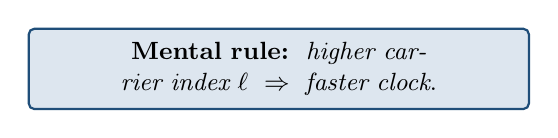
\begin{tikzpicture}
      \node[bluecard,text width=6.0cm] {%
        \textbf{Mental rule:} \,\emph{higher carrier index $\ell$ \;$\Rightarrow$\; faster clock}.
      };
    \end{tikzpicture}
  \end{column}
  \begin{column}{0.58\textwidth}
    \begin{center}
    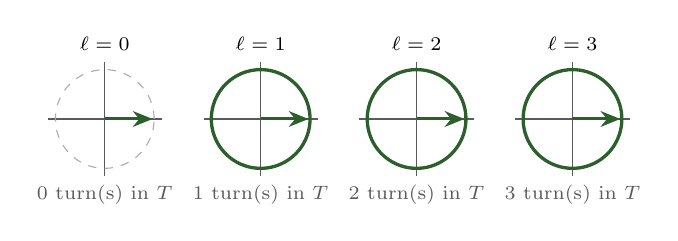
\begin{tikzpicture}[x=0.66cm,y=0.66cm,>=Latex]
      \foreach \k/\dx/\turns in {0/-4.5/0,1/-1.5/1,2/1.5/2,3/4.5/3} {
        \begin{scope}[shift={(\dx,0)}]
          % unit circle + axes
          \draw[inkgray] (-1.1,0) -- (1.1,0);
          \draw[inkgray] (0,-1.1) -- (0,1.1);
          \draw[inkgray!50,dashed] (0,0) circle (0.95);
          % a trail showing how far it has gone at t=T (whole turns)
          \ifnum\k=0
            \draw[accentgreen,line width=1.3pt] (0.95,0) -- (0.95,0);
            \draw[flowarr,color=accentgreen,line width=1.1pt] (0,0) -- (0.92,0);
          \else
            \draw[accentgreen,line width=1.2pt,domain=0:360,samples=80]
              plot ({0.95*cos(\x)},{0.95*sin(\x)});
            \draw[flowarr,color=accentgreen,line width=1.1pt] (0,0) -- (0.92,0);
          \fi
          \node[font=\scriptsize\bfseries] at (0,1.45) {$\ell=\k$};
          \node[font=\scriptsize\color{inkgray}] at (0,-1.45) {\turns\ turn(s) in $T$};
        \end{scope}
      }
    \end{tikzpicture}\\[0.1cm]
    {\scriptsize\itshape\color{inkgray}All clocks start at the same angle and \emph{end at the same angle} (closed loops).}
    \end{center}
  \end{column}
\end{columns}
\end{frame}

% =====================================================================
% 1d. Why orthogonality works (rewritten with clocks)
% =====================================================================
\begin{frame}{1d. Why the FFT can separate carriers}
\stepbadgehdr{1}{“clean OFDM” = closed loops}
\small
\begin{columns}[T,onlytextwidth]
  \begin{column}{0.48\textwidth}
    \vspace{0.15cm}
    \begin{itemize}\setlength{\itemsep}{0.40em}
      \item FFT bin $k$ \emph{listens} by multiplying with a clock spinning \textbf{backward} at rate $k$.
      \item Carrier $\ell$, after that, has rate $\ell-k$ (\emph{leftover spin}).
      \item Average over one symbol $\rightarrow$ closed loops cancel to zero. Only $\ell=k$ survives.
    \end{itemize}
    \[
      c_{k,\ell}^{(0)}
      = \int_0^1 e^{\jj 2\pi(\ell-k)t}\,dt
      =
      \begin{cases}
        1, & \ell = k,\\[0.1em]
        0, & \ell \ne k.
      \end{cases}
    \]
    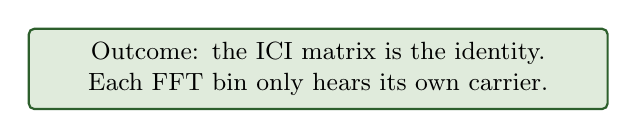
\begin{tikzpicture}
      \node[greencard,text width=7.0cm] {%
        Outcome: the ICI matrix is the identity. Each FFT bin only hears its own carrier.
      };
    \end{tikzpicture}
  \end{column}
  \begin{column}{0.50\textwidth}
    \begin{center}
    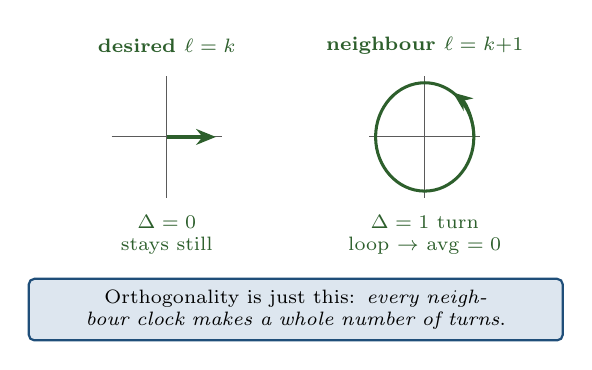
\begin{tikzpicture}[x=0.78cm,y=0.86cm,>=Latex]
      % desired carrier (compact)
      \node[font=\scriptsize\bfseries\color{accentgreen}] at (-2.1,2.05) {desired $\ell=k$};
      \draw[inkgray] (-3.0,0.7) -- (-1.2,0.7);
      \draw[inkgray] (-2.1,-0.20) -- (-2.1,1.60);
      \draw[flowarr,color=accentgreen,line width=1.2pt] (-2.1,0.7) -- (-1.30,0.7);
      \node[font=\scriptsize\color{accentgreen},align=center] at (-2.1,-0.75)
        {$\Delta=0$\\stays still};

      % neighbour, integer turn (compact)
      \node[font=\scriptsize\bfseries\color{accentgreen}] at (2.1,2.05) {neighbour $\ell=k{+}1$};
      \draw[inkgray] (1.2,0.7) -- (3.0,0.7);
      \draw[inkgray] (2.1,-0.20) -- (2.1,1.60);
      \draw[accentgreen,line width=1.1pt] (2.1,0.7) circle (0.80);
      \draw[flowarr,color=accentgreen,line width=1.0pt] (2.90,0.7) arc (0:55:0.80);
      \node[font=\scriptsize\color{accentgreen},align=center] at (2.1,-0.75)
        {$\Delta=1$ turn\\loop $\to$ avg $=0$};

      % bottom callout (narrower)
      \node[bluecard,text width=6.5cm,inner sep=4pt,font=\scriptsize] at (0,-1.85) {%
        Orthogonality is just this: \emph{every neighbour clock makes a whole number of turns}.
      };
    \end{tikzpicture}
    \end{center}
  \end{column}
\end{columns}
\end{frame}

% =====================================================================
% 1e. Bits to tones
% =====================================================================
\begin{frame}{1e. From bits to tone symbols}
\stepbadgehdr{1}{OFDM first turns bits into complex numbers on carriers}
\small
\begin{columns}[T,onlytextwidth]
  \begin{column}{0.48\textwidth}
    Use an $N=8$ toy OFDM symbol.  Bits are first grouped and mapped to
    constellation points:
    \[
      \begin{array}{c|c|c}
        \text{tone } \ell & \text{bits} & d_\ell\\ \hline
        4 & 10 & -1+\jj\\
        5 & 01 & 1-\jj
      \end{array}
    \]
    Then those symbols are placed into frequency bins:
    \[
      \mathbf d=[d_0,d_1,\ldots,d_7].
    \]
    For the next few slides, bin $4$ is the receiver bin we care about.
  \end{column}
  \begin{column}{0.50\textwidth}
    \begin{center}
    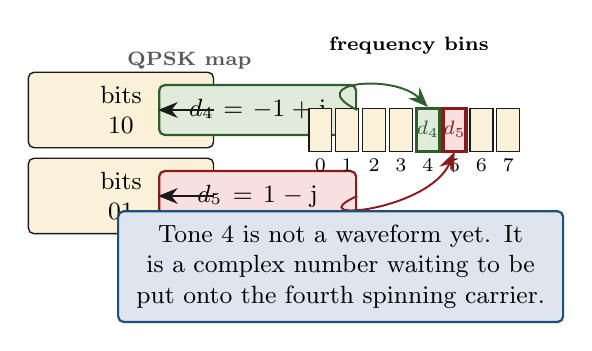
\begin{tikzpicture}[x=0.62cm,y=0.78cm,>=Latex]
      \node[notecard,text width=2.0cm] (b4) at (-3.5,1.2) {bits\\$10$};
      \node[notecard,text width=2.0cm] (b5) at (-3.5,-0.2) {bits\\$01$};
      \node[greencard,text width=2.15cm] (q4) at (-0.7,1.2) {$d_4=-1+\jj$};
      \node[redcard,text width=2.15cm] (q5) at (-0.7,-0.2) {$d_5=1-\jj$};
      \draw[flowarr,color=ink] (b4) -- (q4);
      \draw[flowarr,color=ink] (b5) -- (q5);
      \node[font=\scriptsize\bfseries\color{inkgray}] at (-2.10,2.00) {QPSK map};

      \node[font=\scriptsize\bfseries] at (2.4,2.25) {frequency bins};
      \foreach \i in {0,...,7} {
        \draw[draw=ink,fill=paper,line width=0.45pt] ({0.55*\i+0.35},0.52) rectangle ++(0.47,0.70);
        \node[font=\scriptsize] at ({0.55*\i+0.585},0.30) {\i};
      }
      \draw[draw=accentgreen,line width=1.2pt,fill=grnbg] ({0.55*4+0.35},0.52) rectangle ++(0.47,0.70);
      \draw[draw=accentred,line width=1.2pt,fill=redbg] ({0.55*5+0.35},0.52) rectangle ++(0.47,0.70);
      \node[font=\scriptsize\color{accentgreen}] at ({0.55*4+0.585},0.88) {$d_4$};
      \node[font=\scriptsize\color{accentred}] at ({0.55*5+0.585},0.88) {$d_5$};
      \draw[flowarr,color=accentgreen] (q4.east) .. controls (0.2,1.65) and (2.1,1.80) .. ({0.55*4+0.585},1.25);
      \draw[flowarr,color=accentred] (q5.east) .. controls (0.1,-0.65) and (2.8,-0.45) .. ({0.55*5+0.585},0.52);

      \node[bluecard,text width=5.3cm] at (1.0,-1.35) {%
        Tone $4$ is not a waveform yet. It is a complex number waiting to be put onto the fourth spinning carrier.};
    \end{tikzpicture}
    \end{center}
  \end{column}
\end{columns}
\end{frame}

% =====================================================================
% 1f. IFFT builds the transmit waveform
% =====================================================================
\begin{frame}{1f. The IFFT turns tone symbols into time samples}
\stepbadgehdr{1}{transmission is the sum of all spinning tones}
\small
\begin{columns}[T,onlytextwidth]
  \begin{column}{0.50\textwidth}
    The transmitter takes the tone vector $\mathbf d$ and performs an IFFT:
    \[
      x[n]
      =\frac{1}{8}\sum_{\ell=0}^{7}
        d_\ell e^{\jj2\pi \ell n/8},
      \qquad n=0,\ldots,7.
    \]
    So tone $\ell$ contributes a small rotating sequence:
    \[
      d_\ell e^{\jj2\pi \ell n/8}.
    \]
    In a clean channel, the receiver sees the same samples:
    \[
      r[n]=x[n].
    \]
  \end{column}
  \begin{column}{0.48\textwidth}
    \begin{center}
    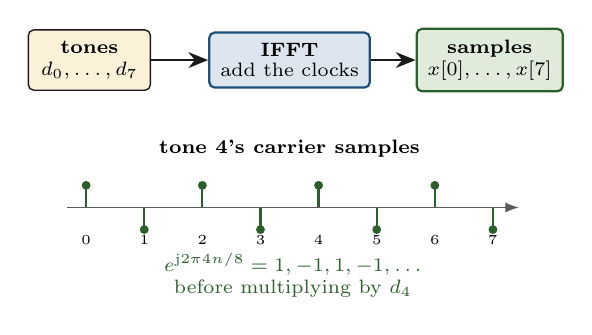
\begin{tikzpicture}[x=0.82cm,y=0.78cm,>=Latex]
      % top row: tones -> IFFT -> samples, with generous gaps
      \node[notecard,minimum width=1.55cm,inner sep=4pt,
            font=\scriptsize,align=center] (tones)
        at (-3.10,1.05) {\textbf{tones}\\$d_0,\ldots,d_7$};
      \node[bluecard,minimum width=1.50cm,inner sep=4pt,
            font=\scriptsize\bfseries,align=center] (ifft) at (0.00,1.05)
        {IFFT\\[-0.1em]\scriptsize\mdseries add the clocks};
      \node[greencard,minimum width=1.85cm,inner sep=4pt,
            font=\scriptsize,align=center] (samples)
        at (3.10,1.05) {\textbf{samples}\\$x[0],\ldots,x[7]$};
      \draw[flowarr,color=ink,line width=0.8pt] (tones.east) -- (ifft.west);
      \draw[flowarr,color=ink,line width=0.8pt] (ifft.east) -- (samples.west);

      % bottom: tone 4 samples stem-plot
      \node[font=\scriptsize\bfseries] at (0,-0.40) {tone 4's carrier samples};
      \foreach \n in {0,...,7} {
        \pgfmathsetmacro{\xx}{-3.15+0.9*\n}
        \pgfmathsetmacro{\yy}{-1.35+0.36*cos(180*\n)}
        \draw[accentgreen,line width=0.8pt] (\xx,-1.35) -- (\xx,\yy);
        \fill[accentgreen] (\xx,\yy) circle (1.6pt);
        \node[font=\tiny] at (\xx,-1.88) {\n};
      }
      \draw[inkgray,->] (-3.45,-1.35) -- (3.55,-1.35);
      \node[font=\scriptsize\color{accentgreen},align=center] at (0.05,-2.45)
        {$e^{\jj2\pi 4 n/8}=1,-1,1,-1,\ldots$\\before multiplying by $d_4$};
    \end{tikzpicture}
    \end{center}
  \end{column}
\end{columns}
\bottomnote{The IFFT builds the transmitted waveform by adding all carriers together.}
\end{frame}

% =====================================================================
% 1g. FFT bin 4 decodes
% =====================================================================
\begin{frame}{1g. FFT bin 4: de-spin and average}
\stepbadgehdr{1}{bin 4 asks: how much fourth carrier is inside $r[n]$?}
\small
\begin{columns}[T,onlytextwidth]
  \begin{column}{0.50\textwidth}
    Receiver bin $4$ multiplies by the opposite fourth carrier and averages:
    \[
      y_4
      =\sum_{n=0}^{7} r[n]e^{-\jj2\pi4n/8}.
    \]
    Substitute the transmitted sum:
    \[
      y_4
      =\sum_{\ell=0}^{7}d_\ell
        \underbrace{\frac{1}{8}\sum_{n=0}^{7}
        e^{\jj2\pi(\ell-4)n/8}}_{\text{how much tone }\ell\text{ enters bin }4}.
    \]
    This bracket is the clean OFDM coupling coefficient $c_{4,\ell}^{(0)}$.
  \end{column}
  \begin{column}{0.48\textwidth}
    \begin{center}
    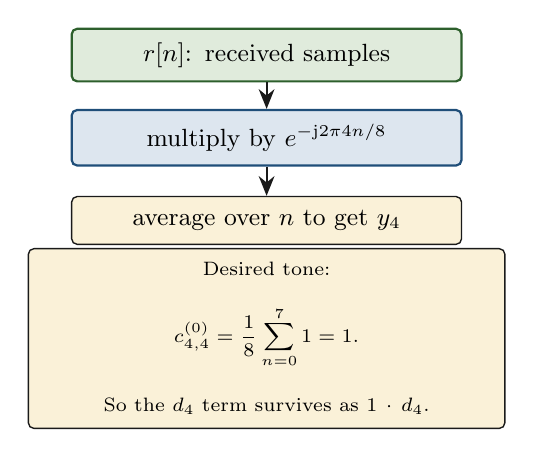
\begin{tikzpicture}[x=1cm,y=1cm,>=Latex]
      \node[greencard,text width=4.6cm] (r) at (0,1.40) {$r[n]$: received samples};
      \node[bluecard,text width=4.6cm] (mix) at (0,0.35) {multiply by $e^{-\jj2\pi4n/8}$};
      \node[notecard,text width=4.6cm] (avg) at (0,-0.70) {average over $n$ to get $y_4$};
      \draw[flowarr,color=ink] (r) -- (mix);
      \draw[flowarr,color=ink] (mix) -- (avg);

      \node[notecard,text width=5.7cm,font=\scriptsize] at (0,-2.20) {%
        Desired tone:
        \[
          c_{4,4}^{(0)}=\frac{1}{8}\sum_{n=0}^{7}1=1.
        \]
        So the $d_4$ term survives as $1\cdot d_4$.};
    \end{tikzpicture}
    \end{center}
  \end{column}
\end{columns}
\bottomnote{FFT bin 4 is one row of the FFT matrix: a matched filter for carrier 4.}
\end{frame}

% =====================================================================
% 1h. Clean numerical example
% =====================================================================
\begin{frame}{1h. Clean numerical example: bin 4 rejects carrier 5}
\stepbadgehdr{1}{now the zero is one entry in FFT row 4}
\small
\begin{columns}[T,onlytextwidth]
  \begin{column}{0.50\textwidth}
    For the neighbour tone $\ell=5$, bin $4$ sees one leftover turn:
    \[
      c_{4,5}^{(0)}
      =\frac{1}{8}\sum_{n=0}^{7}e^{\jj2\pi(5-4)n/8}
      =\frac{1}{8}\sum_{n=0}^{7}e^{\jj2\pi n/8}.
    \]
    The eight arrows are equally spaced around the unit circle, so their sum is zero:
    \[
      c_{4,5}^{(0)}=0,
      \qquad
      d_5\text{ contributes }c_{4,5}^{(0)}d_5=0.
    \]
    Continuous version:
    \(\int_0^1 e^{\jj2\pi(5-4)t}\,dt=0\).
  \end{column}
  \begin{column}{0.48\textwidth}
    \begin{center}
    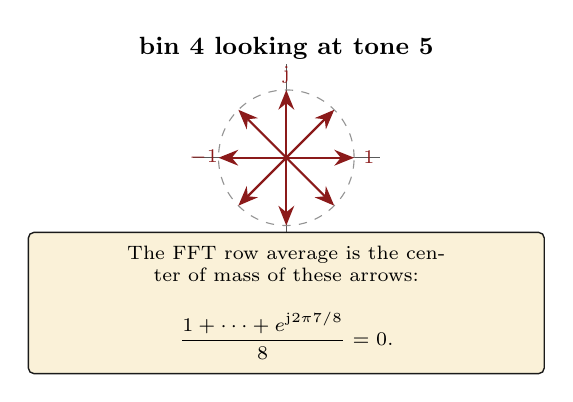
\begin{tikzpicture}[x=0.82cm,y=0.82cm,>=Latex]
      \node[font=\small\bfseries] at (0,2.10) {bin 4 looking at tone 5};
      \draw[inkgray] (-1.45,0.40) -- (1.45,0.40);
      \draw[inkgray] (0,-1.05) -- (0,1.85);
      \draw[inkgray!65,dashed] (0,0.40) circle (1.05);
      \foreach \ang in {0,45,...,315} {
        \draw[flowarr,color=accentred,line width=0.8pt] (0,0.40) -- ++(\ang:1.05);
      }
      \foreach \ang/\lab in {0/$1$,90/$\jj$,180/$-1$,270/$-\jj$} {
        \node[font=\scriptsize\color{accentred}] at ({1.28*cos(\ang)},{0.40+1.28*sin(\ang)}) {\lab};
      }
      \node[notecard,text width=6.2cm,font=\scriptsize] at (0,-1.85) {%
        The FFT row average is the center of mass of these arrows:
        \[
          \frac{1+\cdots+e^{\jj2\pi7/8}}{8}=0.
        \]};
    \end{tikzpicture}
    \end{center}
  \end{column}
\end{columns}
\bottomnote{Doppler breaks this benchmark by making the leftover turn count non-integer.}
\end{frame}

% =====================================================================
% 1i. Common phase is a useful non-example
% =====================================================================
\begin{frame}{1i. A common phase shift does not create ICI}
\stepbadgehdr{1}{same loops, same cancellations}
\small
\begin{columns}[T,onlytextwidth]
  \begin{column}{0.48\textwidth}
    A constant phase shift rotates the \emph{whole} OFDM symbol by the same angle:
    \[
      r(t)=e^{\jj\phi}\sum_\ell d_\ell e^{\jj2\pi f_\ell t}.
    \]
    Bin $k$ still sees
    \[
      y_k=e^{\jj\phi}
      \sum_\ell d_\ell
      \int_0^T e^{\jj2\pi(f_\ell-f_k)t}\,dt
      =e^{\jj\phi}d_k .
    \]
    The constellation rotates, but the off-diagonal carrier terms still integrate to zero.
  \end{column}
  \begin{column}{0.50\textwidth}
    \begin{center}
    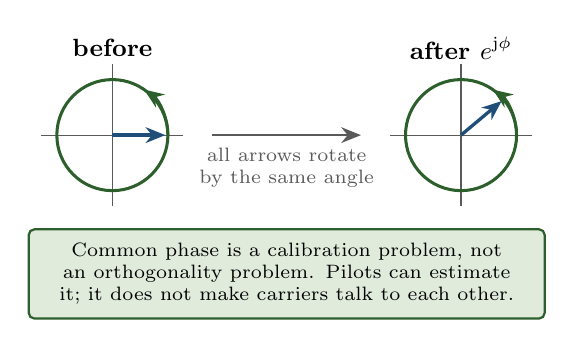
\begin{tikzpicture}[x=0.82cm,y=0.82cm,>=Latex]
      \node[font=\small\bfseries] at (-2.7,2.05) {before};
      \draw[inkgray] (-3.8,0.7) -- (-1.6,0.7);
      \draw[inkgray] (-2.7,-0.4) -- (-2.7,1.8);
      \draw[accentgreen,line width=1.1pt] (-2.7,0.7) circle (0.86);
      \draw[flowarr,color=accentgreen,line width=1.0pt] (-1.84,0.7) arc (0:55:0.86);
      \draw[flowarr,color=accentblue,line width=1.2pt] (-2.7,0.7) -- ++(0.82,0.0);

      \node[font=\small\bfseries] at (2.7,2.05) {after $e^{\jj\phi}$};
      \draw[inkgray] (1.6,0.7) -- (3.8,0.7);
      \draw[inkgray] (2.7,-0.4) -- (2.7,1.8);
      \draw[accentgreen,line width=1.1pt] (2.7,0.7) circle (0.86);
      \draw[flowarr,color=accentgreen,line width=1.0pt] (3.56,0.7) arc (0:55:0.86);
      \draw[flowarr,color=accentblue,line width=1.2pt] (2.7,0.7) -- ++(40:0.82);

      \draw[flowarr,color=inkgray,line width=0.8pt] (-1.15,0.70) -- (1.15,0.70);
      \node[font=\scriptsize\color{inkgray},align=center] at (0,0.20)
        {all arrows rotate\\by the same angle};
      \node[greencard,text width=6.2cm,font=\scriptsize] at (0,-1.45) {%
        Common phase is a calibration problem, not an orthogonality problem. Pilots can estimate it; it does not make carriers talk to each other.};
    \end{tikzpicture}
    \end{center}
  \end{column}
\end{columns}
\end{frame}

% =====================================================================
% 2a. Doppler in everyday life (analogy)
% =====================================================================
\begin{frame}{2a. Doppler is the same thing you hear from a moving siren}
\stepbadgehdr{2}{the everyday analogy}
\small
\begin{columns}[T,onlytextwidth]
  \begin{column}{0.45\textwidth}
    \vspace{0.15cm}
    \begin{itemize}\setlength{\itemsep}{0.45em}
      \item A train whistle is higher \emph{coming toward you} and lower \emph{moving away}.
      \item Same physics underwater: the receiver and transmitter move relative to each other while the OFDM symbol is playing.
      \item Each frequency gets shifted by a tiny amount.
      \item For \emph{wideband} OFDM, high-frequency tones shift more; the whole carrier comb is \textbf{rescaled}.
    \end{itemize}
  \end{column}
  \begin{column}{0.52\textwidth}
    \begin{center}
    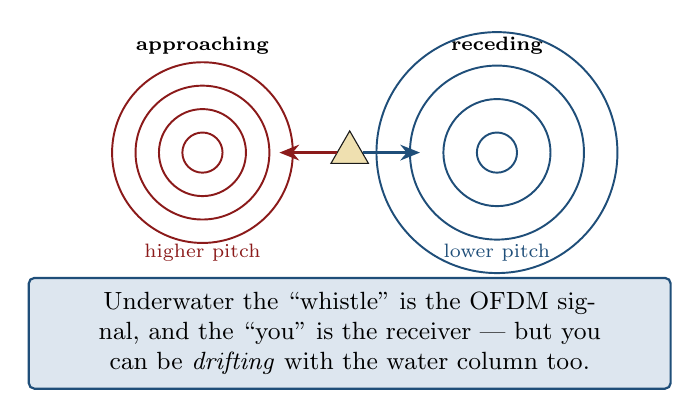
\begin{tikzpicture}[x=0.85cm,y=0.85cm,>=Latex]
      % cartoon siren
      \node[font=\scriptsize\bfseries] at (-2.2,2.10) {approaching};
      \node[font=\scriptsize\bfseries] at (2.2,2.10) {receding};

      % left: tightly-spaced wavefronts
      \foreach \r in {0.30,0.65,1.00,1.35} {
        \draw[accentred,line width=0.7pt] (-2.2,0.5) circle (\r);
      }
      \node[font=\scriptsize\color{accentred}] at (-2.2,-1.0)
        {higher pitch};

      % right: stretched wavefronts
      \foreach \r in {0.30,0.80,1.30,1.80} {
        \draw[accentblue,line width=0.7pt] (2.2,0.5) circle (\r);
      }
      \node[font=\scriptsize\color{accentblue}] at (2.2,-1.0)
        {lower pitch};

      % center: little siren (a triangle)
      \node[regular polygon,regular polygon sides=3,draw=ink,fill=labelbg,
            inner sep=0.5pt,minimum size=0.55cm,font=\tiny] (s) at (0,0.5) {};
      \draw[flowarr,color=accentred,line width=0.8pt] (s) -- (-1.05,0.5);
      \draw[flowarr,color=accentblue,line width=0.8pt] (s) -- (1.05,0.5);

      % under-arrow: ocean version
      \node[bluecard,text width=7.8cm] at (0,-2.20) {%
        Underwater the “whistle” is the OFDM signal, and the “you” is the receiver — but you can be \emph{drifting} with the water column too.};
    \end{tikzpicture}
    \end{center}
  \end{column}
\end{columns}
\end{frame}

% =====================================================================
% 2b. How Doppler is created (math but with intuition first)
% =====================================================================
\begin{frame}{2b. How underwater Doppler shows up in the math}
\stepbadgehdr{2}{wideband: every carrier moves by a different amount}
\small
\begin{columns}[T,onlytextwidth]
  \begin{column}{0.48\textwidth}
    \vspace{0.15cm}
    \textbf{Plain version.}
    Relative motion makes the path length grow or shrink \emph{during} the symbol. The whole waveform gets \emph{time-scaled} by a factor $1+a$:
    \[
      x(t-\tau(t))
      \;=\;
      x\!\big((1+a)\,t - \tau_0\big),
      \quad a=\frac{v}{c_{\mathrm w}} .
    \]
    \textbf{Effect on each carrier.}
    The frequency a receiver sees is
    \[
      f_\ell^{\rx} \;=\; (1+a)\,f_\ell \;+\; \nu,
    \]
    where $\nu$ is any additional common (narrow-band) offset.
    \vspace{0.05cm}
    
\begin{tikzpicture}
      \node[redcard,text width=7.0cm] {%
        Key: \emph{higher $\ell$ moves more}, because the shift $a f_\ell$ grows with $\ell$.
      };
    \end{tikzpicture}
  \end{column}
  \begin{column}{0.50\textwidth}
    \begin{center}
    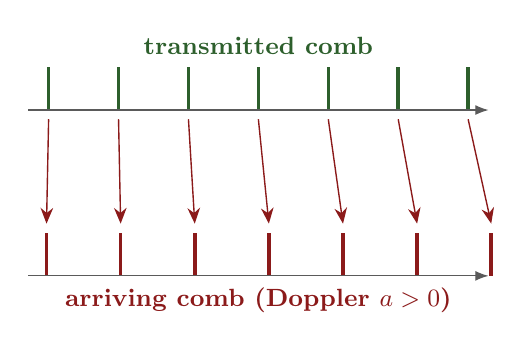
\begin{tikzpicture}[x=0.74cm,y=0.78cm,>=Latex]
      % clean comb on top
      \node[font=\small\bfseries\color{accentgreen}] at (0,2.05) {transmitted comb};
      \foreach \x in {-3.6,-2.4,-1.2,0,1.2,2.4,3.6} {
        \draw[accentgreen,line width=1.3pt] (\x,1.0) -- (\x,1.7);
      }
      \draw[inkgray,->] (-3.95,1.0) -- (3.95,1.0);

      % connecting "Doppler scaling" arrows between the two combs (away from any label)
      \foreach \x in {-3.6,-2.4,-1.2,0,1.2,2.4,3.6} {
        \pgfmathsetmacro{\xs}{\x*1.06+0.18}
        \draw[softarr,color=accentred] (\x,0.85) -- (\xs,-0.85);
      }

      % scaled comb on bottom (label moved BELOW the comb, out of the arrows)
      \foreach \x in {-3.6,-2.4,-1.2,0,1.2,2.4,3.6} {
        \pgfmathsetmacro{\xs}{\x*1.06+0.18}
        \draw[accentred,line width=1.3pt] (\xs,-1.7) -- (\xs,-1.0);
      }
      \draw[inkgray,->] (-3.95,-1.7) -- (3.95,-1.7);
      \node[font=\small\bfseries\color{accentred}] at (0,-2.10) {arriving comb (Doppler $a>0$)};
    \end{tikzpicture}
    \end{center}
    \vspace{-0.10cm}
    \begin{center}
      \scriptsize\itshape\color{inkgray}
      Every comb tooth moves; outer teeth move more than inner ones.
    \end{center}
  \end{column}
\end{columns}
\end{frame}

% =====================================================================
% 2c. What viewed from bin k means
% =====================================================================
\begin{frame}{2c. What ``viewed from bin $k$'' means}
\stepbadgehdr{2}{the FFT changes coordinates before it averages}
\small
Bin $k$ listens by multiplying the received signal by its own backward clock, $e^{-\jj2\pi kt/T}$.
\vspace{0.15cm}

\begin{columns}[T,onlytextwidth]
  \begin{column}{0.50\textwidth}
    \begin{center}
    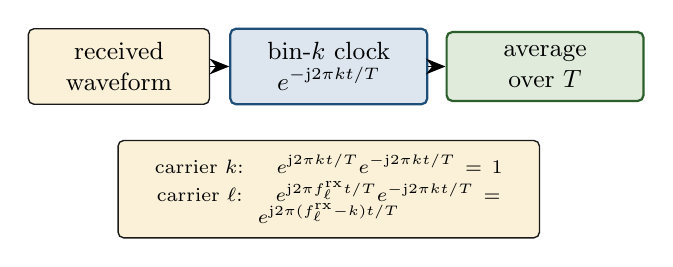
\begin{tikzpicture}[x=0.82cm,y=0.82cm,>=Latex]
      \node[notecard,minimum width=2.3cm] (rx) at (-2.7,0.65) {received\\waveform};
      \node[bluecard,minimum width=2.5cm] (ref) at (0.55,0.65) {bin-$k$ clock\\$e^{-\jj2\pi kt/T}$};
      \node[greencard,minimum width=2.5cm] (avg) at (3.9,0.65) {average\\over $T$};
      \draw[flowarr] (rx) -- (ref);
      \draw[flowarr] (ref) -- (avg);

      \node[notecard,text width=5.0cm,font=\scriptsize] at (0.55,-1.25) {%
        carrier $k$: \quad
        $e^{\jj2\pi kt/T}e^{-\jj2\pi kt/T}=1$\\[0.3em]
        carrier $\ell$: \quad
        $e^{\jj2\pi f_\ell^{\rx}t/T}e^{-\jj2\pi kt/T}
        =e^{\jj2\pi(f_\ell^{\rx}-k)t/T}$};
    \end{tikzpicture}
    \end{center}
  \end{column}
  \begin{column}{0.47\textwidth}
    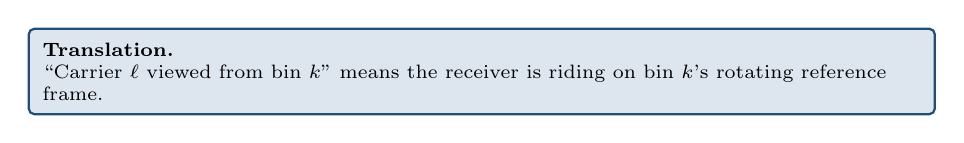
\begin{tikzpicture}
      \node[bluecard,text width=0.92\linewidth,font=\scriptsize,align=left] {%
        \textbf{Translation.}\\
        ``Carrier $\ell$ viewed from bin $k$'' means the receiver is riding on bin $k$'s rotating reference frame.};
    \end{tikzpicture}
    \vspace{0.15cm}
    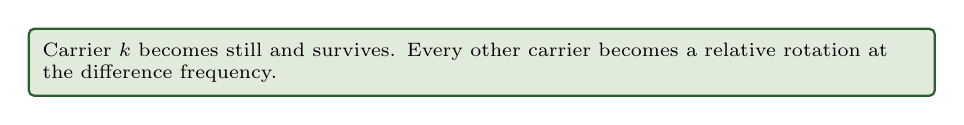
\begin{tikzpicture}
      \node[greencard,text width=0.92\linewidth,font=\scriptsize,align=left] {%
        Carrier $k$ becomes still and survives. Every other carrier becomes a relative rotation at the difference frequency.};
    \end{tikzpicture}
    \vspace{0.15cm}
    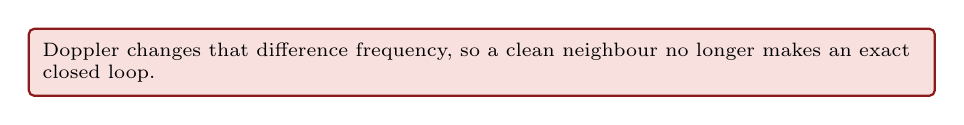
\begin{tikzpicture}
      \node[redcard,text width=0.92\linewidth,font=\scriptsize,align=left] {%
        Doppler changes that difference frequency, so a clean neighbour no longer makes an exact closed loop.};
    \end{tikzpicture}
  \end{column}
\end{columns}
\end{frame}

% =====================================================================
% 2d. Why Delta f times t is a turn count
% =====================================================================
\begin{frame}{2d. Why $\Delta f\,t$ is the fraction of a turn}
\stepbadgehdr{2}{frequency difference $\times$ time = relative turns}
\small
\begin{columns}[T,onlytextwidth]
  \begin{column}{0.46\textwidth}
    Once carrier $\ell$ is viewed from bin $k$, the relative rate is
    \[
      \Delta f=f_\ell^{\rx}-f_k.
    \]
    Frequency is cycles per second. Therefore
    \[
      \underbrace{\Delta f}_{\text{cycles/sec}}
      \times
      \underbrace{t}_{\text{sec}}
      =
      \underbrace{\Delta f\,t}_{\text{cycles}}.
    \]
    The complex exponential turns cycles into angle:
    \[
      e^{\jj2\pi\Delta f t}
      \quad\text{has phase}\quad
      2\pi\Delta f t.
    \]
  \end{column}
  \begin{column}{0.52\textwidth}
    \begin{center}
    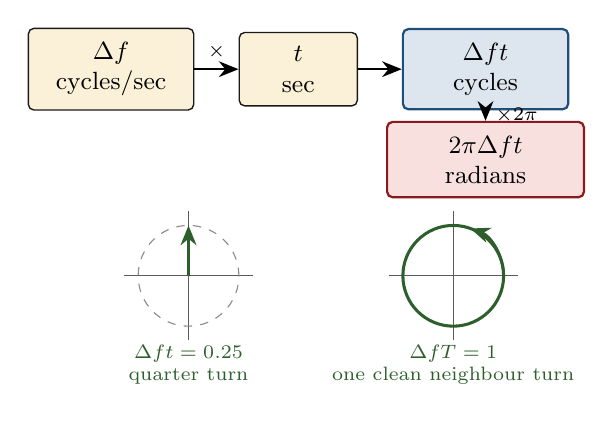
\begin{tikzpicture}[x=0.82cm,y=0.82cm,>=Latex]
      \node[notecard,minimum width=2.1cm] (rate) at (-3.2,1.45) {$\Delta f$\\cycles/sec};
      \node[notecard,minimum width=1.5cm] (time) at (-0.3,1.45) {$t$\\sec};
      \node[bluecard,minimum width=2.1cm] (turns) at (2.6,1.45) {$\Delta f t$\\cycles};
      \node[redcard,minimum width=2.5cm] (phase) at (2.6,0.05) {$2\pi\Delta f t$\\radians};
      \draw[flowarr] (rate) -- node[above,font=\scriptsize] {$\times$} (time);
      \draw[flowarr] (time) -- (turns);
      \draw[flowarr] (turns) -- node[right,font=\scriptsize] {$\times 2\pi$} (phase);

      \begin{scope}[shift={(-2.0,-1.75)}]
        \draw[inkgray] (-1.0,0) -- (1.0,0);
        \draw[inkgray] (0,-1.0) -- (0,1.0);
        \draw[inkgray!70,dashed] (0,0) circle (0.78);
        \draw[flowarr,color=accentgreen,line width=1.2pt] (0,0) -- (0,0.78);
        \node[font=\scriptsize\color{accentgreen},align=center] at (0,-1.38)
          {$\Delta f t=0.25$\\quarter turn};
      \end{scope}
      \begin{scope}[shift={(2.1,-1.75)}]
        \draw[inkgray] (-1.0,0) -- (1.0,0);
        \draw[inkgray] (0,-1.0) -- (0,1.0);
        \draw[accentgreen,line width=1.1pt] (0,0) circle (0.78);
        \draw[flowarr,color=accentgreen,line width=1.0pt] (0.78,0) arc (0:70:0.78);
        \node[font=\scriptsize\color{accentgreen},align=center] at (0,-1.38)
          {$\Delta fT=1$\\one clean neighbour turn};
      \end{scope}
    \end{tikzpicture}
    \end{center}
  \end{column}
\end{columns}
\bottomnote{OFDM spacing is chosen so a clean neighbour has $\Delta fT=1$ full turn. Doppler changes it to $1+\epsilon$, so the loop misses closure.}
\end{frame}

% =====================================================================
% 3a. ICI as an unfinished loop
% =====================================================================
\begin{frame}{3a. ICI is an unfinished de-spinning loop}
\stepbadgehdr{3}{the failed cancellation loop becomes a leakage coefficient}
\small
\begin{columns}[T,onlytextwidth]
  \begin{column}{0.48\textwidth}
    \textbf{No Doppler.}
    Leftover spin between carrier $\ell$ and bin $k$:
    \[
      \Delta_{k,\ell}=\ell-k.
    \]
    Every neighbour gets a whole number of turns, so
    \[
      c_{k,\ell}=\int_0^1 e^{\jj 2\pi \Delta_{k,\ell}t}\,dt = 0,\quad \ell\ne k.
    \]

    \begin{center}
    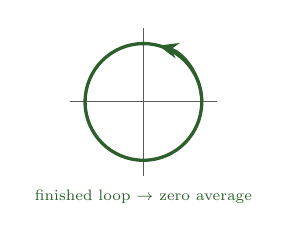
\begin{tikzpicture}[scale=0.78,transform shape]
      \draw[inkgray] (-1.2,0) -- (1.2,0);
      \draw[inkgray] (0,-1.2) -- (0,1.2);
      \draw[accentgreen,line width=1.2pt] (0,0) circle (0.95);
      \draw[flowarr,color=accentgreen,line width=1.0pt] (0.95,0) arc (0:75:0.95);
      \node[font=\scriptsize\color{accentgreen}] at (0,-1.55)
        {finished loop $\to$ zero average};
    \end{tikzpicture}
    \end{center}
  \end{column}
  \begin{column}{0.48\textwidth}
    \textbf{With residual Doppler.}
    Each $\ell$ becomes
    \[
      f_\ell^{\rx}=(1+a)\ell+\nu,\quad
      \Delta_{k,\ell}=(\ell-k)+\nu+a\ell.
    \]
    For neighbour $\ell=k+1$:
    \[
      \Delta_{k,k+1}=1+\nu+a(k+1)
      \;\Rightarrow\; c_{k,k+1}\ne 0.
    \]

    \begin{center}
    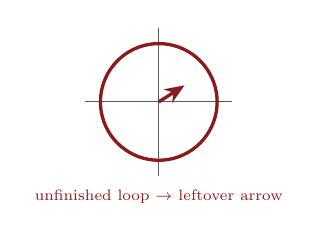
\begin{tikzpicture}[scale=0.78,transform shape]
      \draw[inkgray] (-1.2,0) -- (1.2,0);
      \draw[inkgray] (0,-1.2) -- (0,1.2);
      \draw[accentred,line width=1.2pt,domain=0:445,samples=90]
        plot ({0.95*cos(\x)},{0.95*sin(\x)});
      \draw[flowarr,color=accentred,line width=1.2pt] (0,0) -- (0.42,0.27);
      \node[font=\scriptsize\color{accentred}] at (0,-1.55)
        {unfinished loop $\to$ leftover arrow};
    \end{tikzpicture}
    \end{center}
  \end{column}
\end{columns}
\end{frame}

% =====================================================================
% 3b. Frequency domain (sinc grid)
% =====================================================================
\begin{frame}{3b. Same story in the frequency domain}
\stepbadgehdr{3}{the sinc tails are the leftover arrows}
\small
\begin{columns}[T,onlytextwidth]
  \begin{column}{0.49\textwidth}
    \textbf{Clean OFDM.}\,\, Each carrier is a $\sinc$ centred on its frequency. The FFT samples the spectrum at the bin grid — and lands \emph{on every other carrier's zero}.
    \begin{center}
    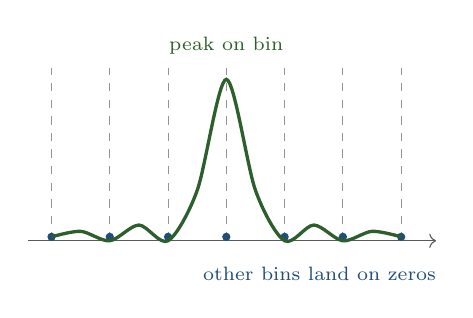
\begin{tikzpicture}[x=0.74cm,y=1.0cm]
      \draw[inkgray,->] (-3.4,0) -- (3.6,0);
      \foreach \k in {-3,-2,-1,0,1,2,3} {
        \draw[inkgray!65,dashed] (\k,0) -- (\k,2.2);
        \fill[accentblue] (\k,0.05) circle (1.5pt);
      }
      \draw[accentgreen,line width=1.2pt,smooth]
        plot coordinates {(-3,0.05)(-2.5,0.12)(-2,0.0)(-1.5,0.20)(-1,0)(-0.5,0.64)(0,2.05)(0.5,0.64)(1,0)(1.5,0.20)(2,0)(2.5,0.12)(3,0.05)};
      \node[font=\scriptsize\color{accentgreen}] at (0,2.48) {peak on bin};
      \node[font=\scriptsize\color{accentblue}] at (1.6,-0.42) {other bins land on zeros};
    \end{tikzpicture}
    \end{center}
  \end{column}
  \begin{column}{0.49\textwidth}
    \textbf{With Doppler.}\,\, The whole carrier sits a fraction of a bin off-grid. The FFT now samples \emph{the tails}, and that is exactly the ICI.
    \begin{center}
    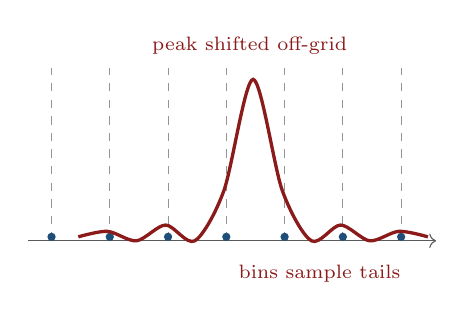
\begin{tikzpicture}[x=0.74cm,y=1.0cm]
      \draw[inkgray,->] (-3.4,0) -- (3.6,0);
      \foreach \k in {-3,-2,-1,0,1,2,3} {
        \draw[inkgray!65,dashed] (\k,0) -- (\k,2.2);
        \fill[accentblue] (\k,0.05) circle (1.5pt);
      }
      \begin{scope}[xshift=0.34cm]
      \draw[accentred,line width=1.2pt,smooth]
        plot coordinates {(-3,0.05)(-2.5,0.12)(-2,0.0)(-1.5,0.20)(-1,0)(-0.5,0.64)(0,2.05)(0.5,0.64)(1,0)(1.5,0.20)(2,0)(2.5,0.12)(3,0.05)};
      \end{scope}
      \node[font=\scriptsize\color{accentred}] at (0.4,2.48) {peak shifted off-grid};
      \node[font=\scriptsize\color{accentred}] at (1.6,-0.42) {bins sample tails};
    \end{tikzpicture}
    \end{center}
  \end{column}
\end{columns}
\bottomnote{The time-domain residual phasor and the frequency-domain sinc tail are the same ICI coefficient seen two ways.}
\end{frame}

% =====================================================================
% 3c. A small numerical example
% =====================================================================
\begin{frame}{3c. A small numerical example you can verify by hand}
\stepbadgehdr{3}{plug the workbench numbers in}
\small
\begin{columns}[T,onlytextwidth]
  \begin{column}{0.49\textwidth}
    \begin{center}
    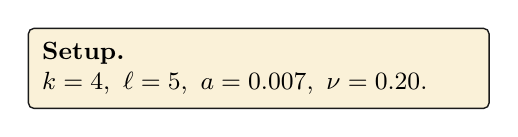
\begin{tikzpicture}
      \node[notecard,text width=5.5cm,align=left] {%
        \textbf{Setup.}\\
        $k=4,\ \ell=5,\ a=0.007,\ \nu=0.20.$
      };
    \end{tikzpicture}
    \end{center}
    \vspace{0.1cm}

    Arrival frequency of carrier 5:
    \[
      f_5^{\rx}=5(1+0.007)+0.20=5.235.
    \]
    Bin 4 sees leftover turns
    \[
      \Delta_{4,5}=f_5^{\rx}-4=1.235.
    \]
    Not an integer $\to$ the loop won't close.
  \end{column}
  \begin{column}{0.49\textwidth}
    Without Doppler:\ $\Delta_{4,5}=1\Rightarrow c_{4,5}=0$.
    \medskip

    With Doppler:
    \[
      c_{4,5}
      =\int_0^1 e^{\jj 2\pi(1.235)t}\,dt
      \approx 0.128+0.117\jj.
    \]
    \[
      |c_{4,5}|\approx 0.173.
    \]
    \begin{center}
    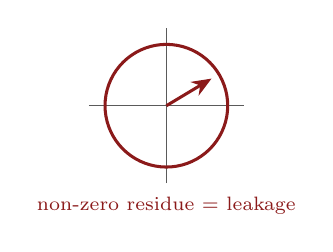
\begin{tikzpicture}[x=0.82cm,y=0.82cm]
      \draw[inkgray] (-1.2,0) -- (1.2,0);
      \draw[inkgray] (0,-1.2) -- (0,1.2);
      \draw[accentred,line width=1.1pt,domain=0:444.6,samples=90]
        plot ({0.95*cos(\x)},{0.95*sin(\x)});
      \draw[flowarr,color=accentred,line width=1.1pt] (0,0) -- (0.70,0.42);
      \node[font=\scriptsize\color{accentred}] at (0,-1.55) {non-zero residue = leakage};
    \end{tikzpicture}
    \end{center}
  \end{column}
\end{columns}
\end{frame}

% =====================================================================
% 3d. From unfinished loop to row term
% =====================================================================
\begin{frame}{3d. How an unfinished loop becomes a row term}
\stepbadgehdr{3}{$c_{k,\ell}$ is both a loop average and a row multiplier}
\small
\begin{columns}[T,onlytextwidth]
  \begin{column}{0.50\textwidth}
    The received waveform contains \emph{all} carriers at once:
    \[
      r(t)=\sum_{\ell} d_\ell
      e^{\jj 2\pi f_\ell^{\rx}t}+n(t).
    \]
    FFT bin $k$ is a linear averaging machine:
    \[
      y_k=\int_0^1 r(t)e^{-\jj 2\pi kt}\,dt.
    \]
    Substitute the sum into the integral:
    \[
      y_k
      =
      \sum_{\ell} d_\ell
      \underbrace{\int_0^1
      e^{\jj 2\pi(f_\ell^{\rx}-k)t}\,dt}_{\substack{\text{loop average}\\c_{k,\ell}}}
      + n_k .
    \]
  \end{column}
	  \begin{column}{0.48\textwidth}
	    \begin{center}
	    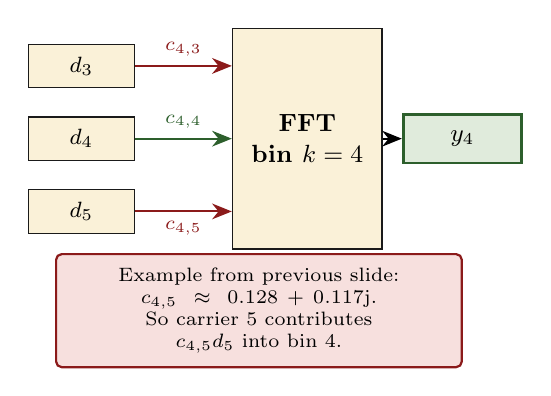
\begin{tikzpicture}[x=0.82cm,y=0.84cm,>=Latex]
	      \node[smallbox,minimum width=1.35cm] (d3) at (-2.55,1.35) {$d_3$};
	      \node[smallbox,minimum width=1.35cm] (d4) at (-2.55,0.25) {$d_4$};
	      \node[smallbox,minimum width=1.35cm] (d5) at (-2.55,-0.85) {$d_5$};

	      \node[draw=ink,fill=paper,line width=0.55pt,align=center,
	        minimum width=1.9cm,minimum height=2.8cm,font=\small\bfseries]
	        (bin) at (0.95,0.25) {FFT\\bin $k=4$};

      \draw[flowarr,color=accentred] (d3) -- node[above,font=\scriptsize] {$c_{4,3}$} (bin.west |- d3);
      \draw[flowarr,color=accentgreen] (d4) -- node[above,font=\scriptsize] {$c_{4,4}$} (bin.west);
      \draw[flowarr,color=accentred] (d5) -- node[below,font=\scriptsize] {$c_{4,5}$} (bin.west |- d5);

	      \node[method,minimum width=1.50cm] (out) at (3.35,0.25) {$y_4$};
	      \draw[flowarr] (bin) -- (out);

	      \node[redcard,text width=4.8cm,font=\scriptsize] at (0.20,-2.35) {%
	        Example from previous slide:\\
	        $c_{4,5}\approx 0.128+0.117\jj$.\\
	        So carrier $5$ contributes $c_{4,5}d_5$ into bin $4$.
	      };
    \end{tikzpicture}
    \end{center}
	  \end{column}
	\end{columns}
	\end{frame}

% =====================================================================
% 3e. Row equation + ICI matrix
% =====================================================================
\begin{frame}{3e. Each FFT row becomes a sum, not a single symbol}
\stepbadgehdr{3}{the ICI matrix is born}
\small
\begin{columns}[T,onlytextwidth]
  \begin{column}{0.45\textwidth}
    Clean OFDM:
    \[
      y_k = c_{k,k}\, d_k + n_k,
      \quad
      c_{k,\ell}=0\ \ (\ell\ne k).
    \]
    Doppler OFDM:
    \[
      y_k = c_{k,k}\, d_k
      +\!\!\sum_{\ell\ne k}\!\! c_{k,\ell}\, d_\ell
      + n_k.
    \]
    The off-diagonal terms are \textbf{ICI} — pieces of \emph{other} symbols inside your bin.
    \vspace{0.20cm}
    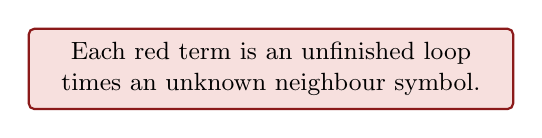
\begin{tikzpicture}
      \node[redcard,text width=5.8cm] {%
        Each red term is an unfinished loop times an unknown neighbour symbol.
      };
    \end{tikzpicture}
  \end{column}
  \begin{column}{0.53\textwidth}
    \begin{center}
    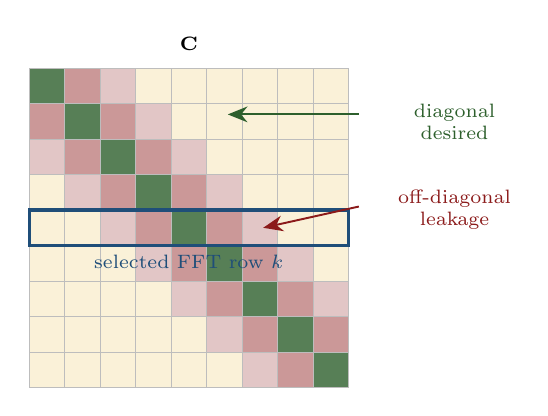
\begin{tikzpicture}[x=0.45cm,y=0.45cm]
      \foreach \r in {0,...,8} {
        \foreach \c in {0,...,8} {
          \pgfmathtruncatemacro{\d}{abs(\r-\c)}
          \ifnum\d=0
            \fill[accentgreen!80] (\c,8-\r) rectangle ++(1,1);
          \else
            \ifnum\d=1
              \fill[accentred!45] (\c,8-\r) rectangle ++(1,1);
            \else
              \ifnum\d=2
                \fill[accentred!25] (\c,8-\r) rectangle ++(1,1);
              \else
                \fill[paper] (\c,8-\r) rectangle ++(1,1);
              \fi
            \fi
          \fi
          \draw[inkgray!40,line width=0.2pt] (\c,8-\r) rectangle ++(1,1);
        }
      }
      \draw[accentblue,line width=1.2pt] (0,4) rectangle (9,5);
      \node[font=\scriptsize\color{accentblue}] at (4.5,3.55) {selected FFT row $k$};
      \node[font=\scriptsize] at (4.5,9.7) {$\mathbf C$};
      \node[font=\scriptsize\color{accentgreen},align=center] at (12.0,7.5)
        {diagonal\\desired};
      \node[font=\scriptsize\color{accentred},align=center] at (12.0,5.0)
        {off-diagonal\\leakage};
      \draw[flowarr,color=accentgreen] (9.3,7.7) -- (5.6,7.7);
      \draw[flowarr,color=accentred] (9.3,5.1) -- (6.6,4.5);
    \end{tikzpicture}
    \end{center}
  \end{column}
\end{columns}
\end{frame}

% =====================================================================
% 3f. ICI as a coupled linear system
% =====================================================================
\begin{frame}{3f. From per-carrier residuals to a coupled system}
\stepbadgehdr{3}{collect the leftover arrows into one matrix}
\small
\begin{columns}[T,onlytextwidth]
  \begin{column}{0.47\textwidth}
    Every transmitted carrier leaves some coefficient in every FFT bin:
    \[
      y_k=\sum_\ell c_{k,\ell}d_\ell+n_k.
    \]
    Stack all bins and all symbols:
    \[
      \mathbf y=\mathbf C\mathbf d+\mathbf n.
    \]
    \vspace{-0.10cm}
    \begin{itemize}\setlength{\itemsep}{0.32em}
      \item \textbf{Static/clean channel:} $\mathbf C$ is diagonal. Each bin sees only its own symbol.
      \item \textbf{Doppler channel:} $\mathbf C$ becomes banded. Each bin sees the desired symbol plus nearby neighbours.
    \end{itemize}

  \end{column}
  \begin{column}{0.51\textwidth}
    \begin{center}
    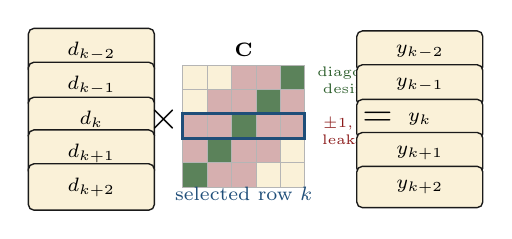
\begin{tikzpicture}[x=0.43cm,y=0.43cm,>=Latex]
      \foreach \i/\lab in {0/$d_{k-2}$,1/$d_{k-1}$,2/$d_k$,3/$d_{k+1}$,4/$d_{k+2}$} {
        \node[notecard,minimum width=1.6cm,font=\scriptsize] (d\i) at (-3.7,{5.2-\i*1.0}) {\lab};
      }

      \foreach \r in {0,...,4} {
        \foreach \c in {0,...,4} {
          \pgfmathtruncatemacro{\dist}{abs(\r-\c)}
          \ifnum\dist=0
            \fill[accentgreen!78] (-1+\c*0.72,1.2+\r*0.72) rectangle ++(0.72,0.72);
          \else
            \ifnum\dist<3
              \fill[accentred!35] (-1+\c*0.72,1.2+\r*0.72) rectangle ++(0.72,0.72);
            \else
              \fill[paper] (-1+\c*0.72,1.2+\r*0.72) rectangle ++(0.72,0.72);
            \fi
          \fi
          \draw[inkgray!45,line width=0.2pt] (-1+\c*0.72,1.2+\r*0.72) rectangle ++(0.72,0.72);
        }
      }
      \node[font=\scriptsize\bfseries] at (0.8,5.25) {$\mathbf C$};
      \node[font=\tiny\color{accentgreen},align=center] at (4.0,4.35) {diagonal\\desired};
      \node[font=\tiny\color{accentred},align=center] at (4.0,2.80) {$\pm1,\pm2$\\leakage};

      \foreach \i/\lab in {0/$y_{k-2}$,1/$y_{k-1}$,2/$y_k$,3/$y_{k+1}$,4/$y_{k+2}$} {
        \node[notecard,minimum width=1.6cm,font=\scriptsize] (y\i) at (6.0,{5.2-\i*1.0}) {\lab};
      }

      \node[font=\Large] at (-1.55,3.20) {$\times$};
      \node[font=\Large] at (4.75,3.20) {$=$};
      \draw[accentblue,line width=1.0pt] (-1,2.64) rectangle (2.6,3.36);
      \node[font=\scriptsize\color{accentblue}] at (0.8,1.0) {selected row $k$};
    \end{tikzpicture}
    \end{center}
  \end{column}
\end{columns}
\end{frame}

% =====================================================================
% 3g. The MMSE benchmark and what it asks of the receiver
% =====================================================================
\begin{frame}{3g. The MMSE benchmark}
\stepbadgehdr{3}{the matrix model's natural linear answer --- and its price}
\small
\begin{columns}[T,onlytextwidth]
  \begin{column}{0.49\textwidth}
    The banded model
    \[
      \mathbf y=\mathbf C\mathbf d+\mathbf n
    \]
    is linear in the data, so the minimum-mean-square-error estimator follows
    by inspection:
    \[
      \widehat{\mathbf d}_{\rm MMSE}
      =
      \bigl(\mathbf C^{\mathsf H}\mathbf C+\sigma_n^2\mathbf I\bigr)^{-1}
      \mathbf C^{\mathsf H}\mathbf y .
    \]

    On paper this closes the chapter: no linear receiver does better once
    $\mathbf C$ and $\sigma_n^2$ are known.

    \vspace{0.30em}
    The work has only moved.  Each block now demands a coupling matrix
    estimated from the pilots, and a coupled inverse solved before the next
    block arrives --- exactly the budget an underwater link cannot spend.
  \end{column}
  \begin{column}{0.49\textwidth}
    \begin{center}
    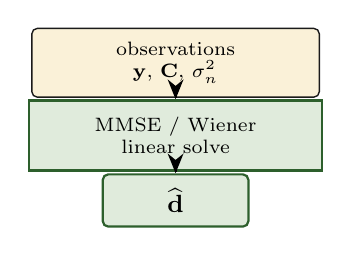
\begin{tikzpicture}[x=0.78cm,y=0.66cm,>=Latex]
      \node[notecard,text width=3.30cm,font=\scriptsize,align=center] (obs) at (0,2.55)
        {observations\\$\mathbf y$,\ $\mathbf C$,\ $\sigma_n^2$};
      \node[method,text width=3.30cm,font=\scriptsize,align=center] (mmse) at (0,1.15)
        {MMSE / Wiener\\linear solve};
      \node[greencard,minimum width=1.85cm,align=center] (dhat) at (0,-0.10)
        {$\widehat{\mathbf d}$};
      \draw[flowarr] (obs) -- (mmse);
      \draw[flowarr] (mmse) -- (dhat);
    \end{tikzpicture}
    \end{center}

    \vspace{0.10em}
    \begin{center}
    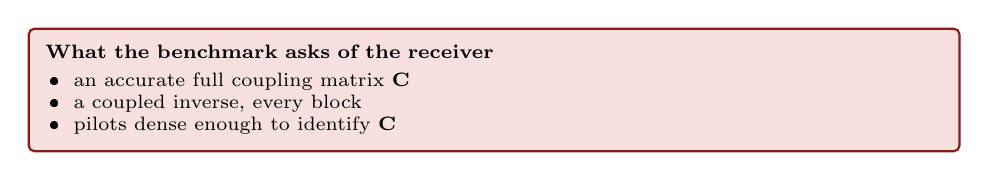
\begin{tikzpicture}
      \node[redcard,text width=0.94\linewidth,font=\scriptsize,align=left,
            inner sep=6pt] {%
        \textbf{What the benchmark asks of the receiver}\\[2pt]
        \,\textbullet\; an accurate full coupling matrix $\mathbf C$\\
        \,\textbullet\; a coupled inverse, every block\\
        \,\textbullet\; pilots dense enough to identify $\mathbf C$
      };
    \end{tikzpicture}
    \end{center}

    \vspace{0.20em}
    \centerline{\itshape\scriptsize\color{inkgray}
      Slide 3h relaxes each of these in turn.}
  \end{column}
\end{columns}
\end{frame}

% =====================================================================
% 3h. Bridge from matrix solve to partial FFT
% =====================================================================
\begin{frame}{3h. The missing step: partial FFT is a stopped FFT}
\stepbadgehdr{3}{same samples, same bin, but do not add all four pieces yet}
\small
\begin{columns}[T,onlytextwidth]
  \begin{column}{0.47\textwidth}
    After bin-$k$ demodulation, every received sample becomes
    \[
      q_k[n]=r[n]\,e^{-\jj2\pi kn/N}.
    \]

    The usual FFT bin adds the whole row:
    \[
      y_k=\sum_{n=0}^{N-1}q_k[n].
    \]

    Partial FFT adds the same row in pieces:
    \[
      z_{m,k}=\sum_{n\in\mathcal S_m}q_k[n],
      \qquad
      \mathbf z_k=
      \begin{bmatrix}z_{0,k}\\z_{1,k}\\z_{2,k}\\z_{3,k}\end{bmatrix}.
    \]

  \end{column}
  \begin{column}{0.51\textwidth}
    \begin{center}
    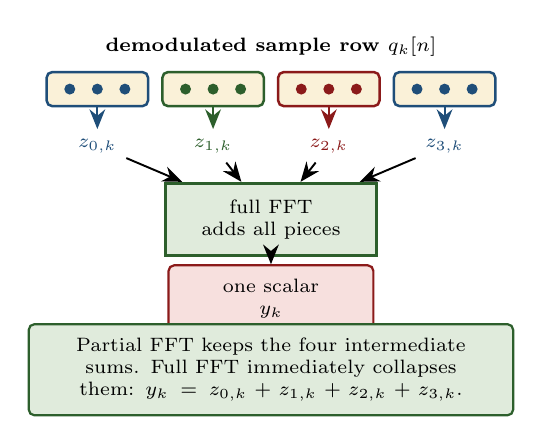
\begin{tikzpicture}[x=0.70cm,y=0.72cm,>=Latex]
      \node[font=\scriptsize\bfseries] at (0,3.00) {demodulated sample row $q_k[n]$};
      \foreach \m/\x/\c in {0/-3.15/accentblue,1/-1.05/accentgreen,2/1.05/accentred,3/3.15/accentblue} {
        \draw[fill=paper,draw=\c,line width=0.9pt,rounded corners=2pt] (\x-0.92,1.95) rectangle (\x+0.92,2.55);
        \foreach \i in {-0.50,0,0.50} {
          \node[circle,fill=\c,inner sep=1.4pt] at (\x+\i,2.25) {};
        }
        \node[font=\scriptsize\color{\c}] (z\m) at (\x,1.25) {$z_{\m,k}$};
        \draw[flowarr,color=\c] (\x,1.95) -- (z\m);
      }

      \node[method,text width=2.25cm,font=\scriptsize,align=center] (full) at (0,-0.05)
        {full FFT\\adds all pieces};
      \foreach \m in {0,1,2,3} {
        \draw[flowarr] (z\m) -- (full);
      }
      \node[redcard,text width=2.25cm,font=\scriptsize,align=center] (yk) at (0,-1.45)
        {one scalar\\$y_k$};
      \draw[flowarr] (full) -- (yk);

      \node[greencard,text width=5.80cm,font=\scriptsize,align=center] at (0,-2.70) {%
        Partial FFT keeps the four intermediate sums.
        Full FFT immediately collapses them:
        \(y_k=z_{0,k}+z_{1,k}+z_{2,k}+z_{3,k}\).};
    \end{tikzpicture}
    \end{center}
  \end{column}
\end{columns}
\end{frame}

% =====================================================================
% 3i. Why the mixture has vector fingerprints
% =====================================================================
\begin{frame}{3i. One branch: the same sum splits by tone}
\stepbadgehdr{3}{linearity means wanted and leak pass through the branch separately}
\small
\begin{columns}[T,onlytextwidth]
  \begin{column}{0.47\textwidth}
    Suppose the received samples contain the wanted tone and one leaking tone:
    \[
      r[n]=d_k a_k[n]+d_\ell a_\ell[n]+\cdots
    \]
    where $a_\ell[n]$ means ``tone $\ell$ after channel and Doppler.''

    Branch $m$ is just a sum over its own segment $\mathcal S_m$:
    \[
      z_{m,k}
      =\sum_{n\in\mathcal S_m} r[n]e^{-\jj2\pi kn/N}.
    \]
  \end{column}
  \begin{column}{0.51\textwidth}
    Substitute $r[n]$ into that branch:
    \[
    \begin{aligned}
      z_{m,k}
      &=
      \underbrace{\sum_{n\in\mathcal S_m}
        a_k[n]e^{-\jj2\pi kn/N}}_{h_{m;k,k}}d_k\\
      &\quad+
      \underbrace{\sum_{n\in\mathcal S_m}
        a_\ell[n]e^{-\jj2\pi kn/N}}_{h_{m;k,\ell}}d_\ell
      +\cdots .
    \end{aligned}
    \]
    \begin{center}
    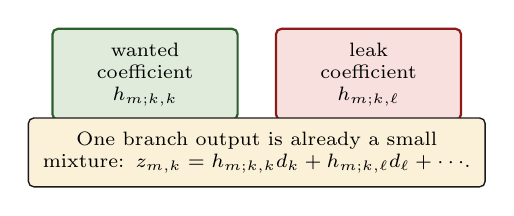
\begin{tikzpicture}[x=0.86cm,y=0.62cm,>=Latex]
      \node[greencard,text width=2.00cm,font=\scriptsize,align=center] (want) at (-1.65,0)
        {wanted\\coefficient\\$h_{m;k,k}$};
      \node[redcard,text width=2.00cm,font=\scriptsize,align=center] (leak) at (1.65,0)
        {leak\\coefficient\\$h_{m;k,\ell}$};
      \node[notecard,text width=5.45cm,font=\scriptsize,align=center] at (0,-1.60) {%
        One branch output is already a small mixture:
        \(z_{m,k}=h_{m;k,k}d_k+h_{m;k,\ell}d_\ell+\cdots\).};
    \end{tikzpicture}
    \end{center}
  \end{column}
\end{columns}
\end{frame}

% =====================================================================
% 3j. Stack branches, then compare with full FFT
% =====================================================================
\begin{frame}{3j. Stack four branches: now the leak has a shape}
\stepbadgehdr{3}{the vector is just four branch equations placed on top of each other}
\footnotesize
\begin{columns}[T,onlytextwidth]
  \begin{column}{0.52\textwidth}
    Each segment gives one equation:
    \[
      z_{m,k}=h_{m;k,k}d_k+h_{m;k,\ell}d_\ell+\cdots .
    \]

    Stack $m=0,1,2,3$:
    \[
      \mathbf z_k=
      \mathbf h_{k,k}d_k+\mathbf h_{k,\ell}d_\ell+\cdots
    \]
    where
    \[
      \mathbf h_{k,\ell}=
      \begin{bmatrix}
      h_{0;k,\ell}\\h_{1;k,\ell}\\h_{2;k,\ell}\\h_{3;k,\ell}
      \end{bmatrix}.
    \]
  \end{column}
  \begin{column}{0.46\textwidth}
    Full FFT adds the four rows first:
    \[
      y_k=\sum_{m=0}^{3} z_{m,k}.
    \]
    So each vector fingerprint becomes one scalar:
    \[
      c_{k,\ell}=\sum_{m=0}^{3}h_{m;k,\ell}.
    \]
    Therefore
    \[
      y_k=c_{k,k}d_k+c_{k,\ell}d_\ell+\cdots .
    \]

    \begin{center}
    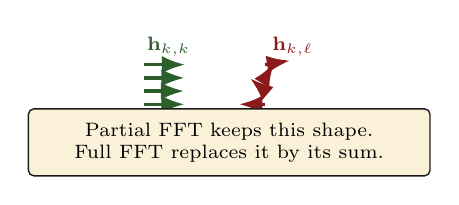
\begin{tikzpicture}[x=0.70cm,y=0.42cm,>=Latex]
      \foreach \m/\y/\len in {0/1.30/0.75,1/0.90/0.74,2/0.50/0.73,3/0.10/0.74} {
        \draw[accentgreen,line width=1.2pt,-Latex] (-1.65,\y) -- ++(\len,0);
        \draw[accentred,line width=1.2pt,-Latex] (0.55,\y) -- ++({0.47*cos(55*\m+15)},{0.47*sin(55*\m+15)});
      }
      \node[font=\scriptsize\bfseries\color{accentgreen}] at (-1.20,1.85) {$\mathbf h_{k,k}$};
      \node[font=\scriptsize\bfseries\color{accentred}] at (1.05,1.85) {$\mathbf h_{k,\ell}$};
      \node[notecard,text width=4.75cm,font=\scriptsize,align=center] at (-0.10,-1.05) {%
        Partial FFT keeps this shape.
        Full FFT replaces it by its sum.};
    \end{tikzpicture}
    \end{center}
  \end{column}
\end{columns}
\end{frame}

% =====================================================================
% 4a. Why one long FFT is fragile
% =====================================================================
\begin{frame}{4a. Why one long FFT is the fragile step}
\stagefourhdr{1}{full FFT is a fixed, equal-weight combiner}
\small
\begin{columns}[T,onlytextwidth]
  \begin{column}{0.48\textwidth}
    Use the branch-vector view from slide 3j:
    \[
      \mathbf z_k=[z_{0,k},z_{1,k},z_{2,k},z_{3,k}]^{\mathsf T}.
    \]
    A full FFT is what you get if the receiver secretly uses the
    \textbf{fixed equal weights}
    \[
      \mathbf w_{\rm full}
      =
      \frac{1}{4}
      \begin{bmatrix}1\\1\\1\\1\end{bmatrix}.
    \]
    Therefore
    \[
      y_k^{\rm full}
      =
      \mathbf w_{\rm full}^{\mathsf H}\mathbf z_k .
    \]

    \vspace{-0.15cm}
    Substitute the desired and leak fingerprints:
    \[
      y_k^{\rm full}
      =
      \underbrace{\mathbf w_{\rm full}^{\mathsf H}\mathbf h_{k,k}}_{\text{wanted}}
      d_k
      +
      \underbrace{\mathbf w_{\rm full}^{\mathsf H}\mathbf h_{k,\ell}}_{\text{leak}}
      d_\ell+\cdots .
    \]
  \end{column}
  \begin{column}{0.50\textwidth}
    \begin{center}
    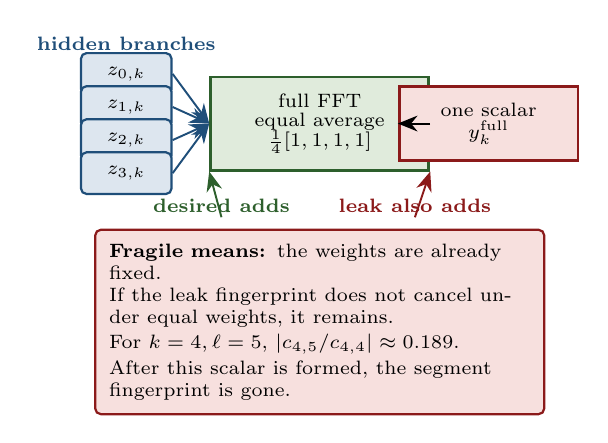
\begin{tikzpicture}[x=0.78cm,y=0.70cm,>=Latex]
      \foreach \m/\y in {0/2.95,1/2.35,2/1.75,3/1.15} {
        \node[bluecard,minimum width=1.15cm,font=\scriptsize] (z\m) at (-3.25,\y) {$z_{\m,k}$};
      }
      \node[font=\scriptsize\bfseries\color{accentblue}] at (-3.25,3.50)
        {hidden branches};

      \node[method,text width=2.35cm,font=\scriptsize] (avg) at (-0.10,2.05) {%
        full FFT\\[-0.1em]
        equal average\\[-0.1em]
        $\frac{1}{4}[1,1,1,1]$};
      \node[issue,text width=1.85cm,font=\scriptsize] (out) at (2.65,2.05)
        {one scalar\\$y_k^{\rm full}$};

      \foreach \m in {0,1,2,3} {
        \draw[flowarr,color=accentblue] (z\m.east) -- (avg.west);
      }
      \draw[flowarr] (avg) -- (out);

      \node[font=\scriptsize\bfseries\color{accentgreen}] at (-1.70,0.55)
        {desired adds};
      \node[font=\scriptsize\bfseries\color{accentred}] at (1.45,0.55)
        {leak also adds};
      \draw[flowarr,color=accentgreen] (-1.70,0.35) -- (avg.south west);
      \draw[flowarr,color=accentred] (1.45,0.35) -- (avg.south east);

      \node[redcard,text width=5.35cm,font=\scriptsize,align=left] at (-0.10,-1.55) {%
        \textbf{Fragile means:} the weights are already fixed.\\
        If the leak fingerprint does not cancel under equal weights, it remains.\\[0.15em]
        For $k=4,\ell=5$, $|c_{4,5}/c_{4,4}|\approx0.189$.\\[0.15em]
        After this scalar is formed, the segment fingerprint is gone.};
    \end{tikzpicture}
    \end{center}
  \end{column}
\end{columns}
\end{frame}

% =====================================================================
% 4b. Partial FFT keeps short-window views
% =====================================================================
\begin{frame}{4b. Partial FFT: keep the pieces, then combine}
\stagefourhdr{2}{the fix: split before the final average}
\small
\begin{columns}[T,onlytextwidth]
  \begin{column}{0.46\textwidth}
    Slide 4a lost the time pattern. Partial FFT stores it as several local FFT outputs.

    \vspace{0.30em}
    Split one symbol into $M=4$ shorter windows:
    \[
      z_{m,k}
      =\frac{1}{\Delta T}
      \!\int_{m\Delta T}^{(m+1)\Delta T}\!\!
      r(t)\, e^{-\jj 2\pi kt}\, dt.
    \]

    \vspace{0.20em}
    Stack them into a branch vector
    \[
      \vY_k = [z_{0,k},\, z_{1,k},\, z_{2,k},\, z_{3,k}]\T .
    \]

    \vspace{0.10em}
    {\scriptsize The branch vector keeps how the symbol \emph{changed} across $T$ — exactly the information the full FFT averaged away.}
	  \end{column}
  \begin{column}{0.52\textwidth}
    \begin{center}
    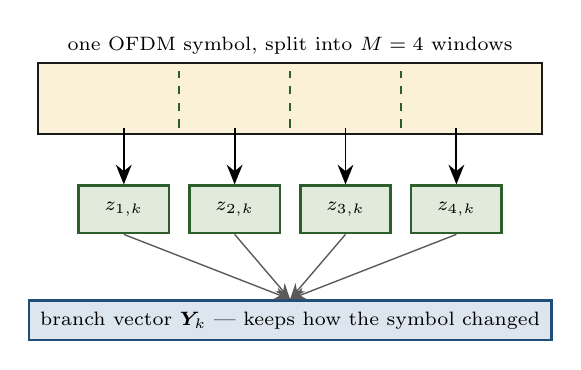
\begin{tikzpicture}[x=0.88cm,y=0.88cm,>=Latex]
      % the symbol window
      \node[draw=ink,fill=paper,line width=0.5pt,
            minimum width=6.4cm,minimum height=0.90cm] (sym) at (0,1.60) {};
      \node[font=\scriptsize,anchor=south] at (0,2.10) {one OFDM symbol, split into $M=4$ windows};
      % splitter ticks INSIDE the box only
      \foreach \x in {-1.6,0.0,1.6} {
        \draw[accentgreen,line width=0.8pt,dashed] (\x,1.18) -- (\x,2.00);
      }
      % four short-window FFT outputs
      \foreach \i/\x in {1/-2.4,2/-0.8,3/0.8,4/2.4} {
        \node[method,minimum width=1.15cm,font=\scriptsize] (b\i) at (\x,0.00)
          {$z_{\i,k}$};
        \draw[flowarr] (\x,1.18) -- (b\i.north);
      }
      % branch vector card
      \node[idea,minimum width=5.0cm,font=\scriptsize,inner sep=4pt] (vec) at (0,-1.60)
        {branch vector $\vY_k$ — keeps how the symbol changed};
      \foreach \i in {1,2,3,4} {
        \draw[softarr] (b\i.south) -- (vec.north);
      }
    \end{tikzpicture}
    \end{center}
  \end{column}
\end{columns}
\end{frame}

% =====================================================================
% 4b'. Numerical check of the four partial-FFT outputs
% =====================================================================
\begin{frame}{4b\textquotesingle. The four pieces, in numbers}
\stagefourhdr{2}{check: an equal average reconstructs the full-FFT leak}
\small
\begin{columns}[T,onlytextwidth]
  \begin{column}{0.48\textwidth}
    For the leakage path $k=4$, $\ell=5$ (the carrier we are tracking from earlier slides), the four short-window coefficients are
    \[
      \begin{aligned}
        c^{(1)} &= \phantom{-}0.481 + 0.701\jj,\\
        c^{(2)} &= -0.828 + 0.195\jj,\\
        c^{(3)} &= \phantom{-}0.117 - 0.842\jj,\\
        c^{(4)} &= \phantom{-}0.744 + 0.413\jj.
      \end{aligned}
    \]
    Each $c^{(m)}$ is the leakage contribution \emph{measured within window $m$}.
  \end{column}
  \begin{column}{0.48\textwidth}
    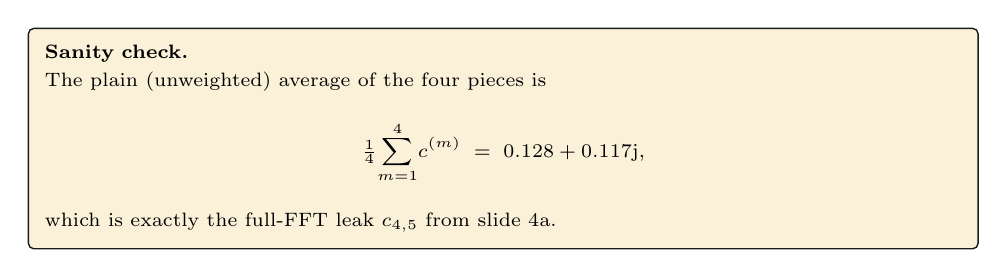
\begin{tikzpicture}
      \node[notecard,text width=0.96\linewidth,inner sep=6pt,
            align=left,font=\scriptsize] {%
        \textbf{Sanity check.}\\[0.25em]
        The plain (unweighted) average of the four pieces is
        \[
          \tfrac{1}{4}\!\sum_{m=1}^{4}\! c^{(m)}
          \;=\; 0.128 + 0.117\jj,
        \]
        which is exactly the full-FFT leak $c_{4,5}$ from slide 4a.
      };
    \end{tikzpicture}

    \vspace{0.30cm}
    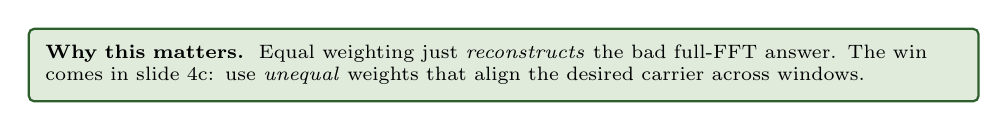
\begin{tikzpicture}
      \node[greencard,text width=0.96\linewidth,inner sep=6pt,
            align=left,font=\scriptsize] {%
        \textbf{Why this matters.}\,
        Equal weighting just \emph{reconstructs} the bad full-FFT answer. The win comes in slide 4c: use \emph{unequal} weights that align the desired carrier across windows.
      };
    \end{tikzpicture}
  \end{column}
\end{columns}
\bottomnote{The four $c^{(m)}$ values are the raw material for everything that follows.}
\end{frame}

% =====================================================================
% 4c. Weights align desired
% =====================================================================
\begin{frame}{4c. Combining weights line up the desired carrier}
\stagefourhdr{3}{first job: rotate the desired pieces so they all point the same way}
\small
\begin{columns}[T,onlytextwidth]
  \begin{column}{0.48\textwidth}
    Each branch contains a desired piece $c_{m,k,k}d_k$ plus leakage.
    Pick complex weights $w_{m,k}$ and form
    \[
      \widetilde{y}_k
      =\frac{1}{M}\sum_{m=0}^{M-1} w_{m,k}\,z_{m,k}.
    \]
    Choose $w_{m,k}$ so that $w_{m,k}\, c_{m,k,k}$ all point the \emph{same direction}.

    \vspace{0.12cm}
    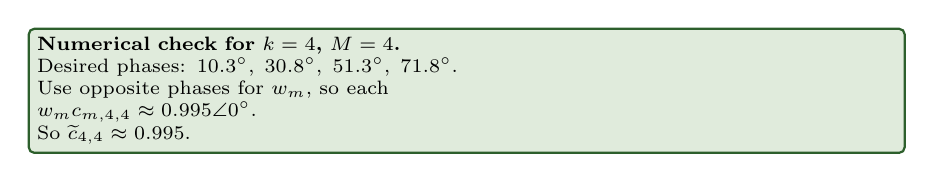
\begin{tikzpicture}
      \node[greencard,text width=0.90\linewidth,inner sep=3pt,font=\scriptsize,align=left] {%
        \textbf{Numerical check for $k=4$, $M=4$.}\\
        Desired phases: $10.3^\circ,\;30.8^\circ,\;51.3^\circ,\;71.8^\circ$.\\
        Use opposite phases for $w_m$, so each\\
        $w_m c_{m,4,4}\approx 0.995\angle 0^\circ$.\\
        So $\widetilde c_{4,4}\approx 0.995$.
      };
    \end{tikzpicture}
  \end{column}
  \begin{column}{0.50\textwidth}
    \begin{center}
    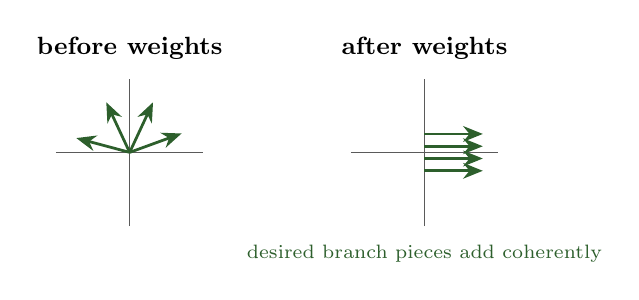
\begin{tikzpicture}[x=0.78cm,y=0.78cm,>=Latex]
      \node[font=\small\bfseries] at (-2.4,2.30) {before weights};
      \draw[inkgray] (-3.6,0.6) -- (-1.2,0.6);
      \draw[inkgray] (-2.4,-0.6) -- (-2.4,1.8);
      \foreach \ang in {20,65,115,165} {
        \draw[flowarr,color=accentgreen,line width=1.0pt] (-2.4,0.6) -- ++(\ang:0.9);
      }

      \node[font=\small\bfseries] at (2.4,2.30) {after weights};
      \draw[inkgray] (1.2,0.6) -- (3.6,0.6);
      \draw[inkgray] (2.4,-0.6) -- (2.4,1.8);
      \foreach \y in {0.30,0.50,0.70,0.90} {
        \draw[flowarr,color=accentgreen,line width=1.0pt] (2.4,\y) -- ++(0.95,0);
      }
      \node[font=\scriptsize\color{accentgreen},align=center] at (2.4,-1.05)
        {desired branch pieces add coherently};
    \end{tikzpicture}
    \end{center}
  \end{column}
\end{columns}
\end{frame}

% =====================================================================
% 4d. Same weights spoil leakage
% =====================================================================
\begin{frame}{4d. The same weights make the leakage less coherent}
\stagefourhdr{4}{second job: scramble the unwanted pieces}
\small
\begin{columns}[T,onlytextwidth]
  \begin{column}{0.48\textwidth}
    After combining, the effective coefficient is
    \[
      \widetilde{c}_{k,\ell}
      =\frac{1}{M}\sum_{m=0}^{M-1} w_{m,k}\, c_{m,k,\ell}.
    \]
    For $\ell=k$, weights were chosen so terms add. For $\ell\ne k$, the leakage terms typically have \emph{different phases per branch}, so after the same alignment they partly cancel.

    \vspace{0.2cm}
    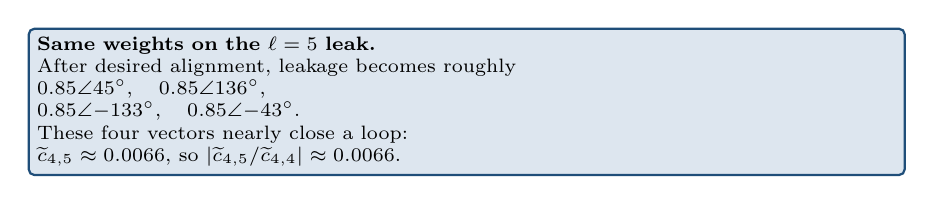
\begin{tikzpicture}
      \node[bluecard,text width=0.90\linewidth,inner sep=3pt,font=\scriptsize,align=left] {%
        \textbf{Same weights on the $\ell=5$ leak.}\\
        After desired alignment, leakage becomes roughly\\
        $0.85\angle 45^\circ,\quad 0.85\angle 136^\circ,$\\
        $0.85\angle {-133}^\circ,\quad 0.85\angle {-43}^\circ.$\\
        These four vectors nearly close a loop:\\
        $\widetilde c_{4,5}\approx 0.0066$, so
        $|\widetilde c_{4,5}/\widetilde c_{4,4}|\approx 0.0066$.
      };
    \end{tikzpicture}
  \end{column}
  \begin{column}{0.50\textwidth}
    \begin{center}
    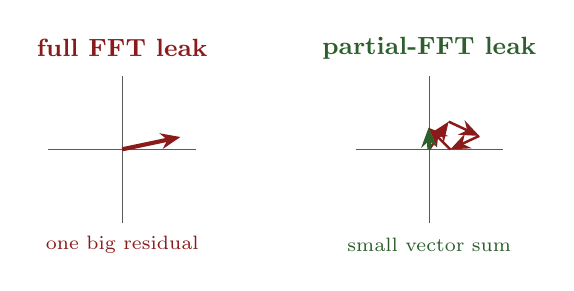
\begin{tikzpicture}[x=0.78cm,y=0.78cm,>=Latex]
      \node[font=\small\bfseries\color{accentred}] at (-2.5,2.25) {full FFT leak};
      \draw[inkgray] (-3.7,0.6) -- (-1.3,0.6);
      \draw[inkgray] (-2.5,-0.6) -- (-2.5,1.8);
      \draw[flowarr,color=accentred,line width=1.5pt] (-2.5,0.6) -- ++(0.95,0.20);
      \node[font=\scriptsize\color{accentred}] at (-2.5,-0.95) {one big residual};

      \node[font=\small\bfseries\color{accentgreen}] at (2.5,2.25) {partial-FFT leak};
      \draw[inkgray] (1.3,0.6) -- (3.7,0.6);
      \draw[inkgray] (2.5,-0.6) -- (2.5,1.8);
      \coordinate (p0) at (2.5,0.6);
      \coordinate (p1) at ($(p0)+(55:0.55)$);
      \coordinate (p2) at ($(p1)+(-25:0.55)$);
      \coordinate (p3) at ($(p2)+(205:0.52)$);
      \coordinate (p4) at ($(p3)+(135:0.50)$);
      \draw[flowarr,color=accentred,line width=0.9pt] (p0) -- (p1);
      \draw[flowarr,color=accentred,line width=0.9pt] (p1) -- (p2);
      \draw[flowarr,color=accentred,line width=0.9pt] (p2) -- (p3);
      \draw[flowarr,color=accentred,line width=0.9pt] (p3) -- (p4);
      \draw[flowarr,color=accentgreen,line width=1.4pt] (p0) -- (p4);
      \node[font=\scriptsize\color{accentgreen}] at (2.5,-0.95) {small vector sum};
    \end{tikzpicture}
    \end{center}
  \end{column}
\end{columns}
\end{frame}

% =====================================================================
% 4e. Before / after the row
% =====================================================================
\begin{frame}{4e. Before and after, on the same row}
\stagefourhdr{5}{the diagonal stays loud, many leaks get quiet}
\small
\begin{columns}[T,onlytextwidth]
  \begin{column}{0.49\textwidth}
    \textbf{Full FFT, one-tap corrected.}
    \[
      \frac{y_k}{c_{k,k}}
      = d_k
      +\!\!\sum_{\ell\ne k}\!\!
      \frac{c_{k,\ell}}{c_{k,k}}\, d_\ell
      +\tilde n_k.
    \]
    Example: $|c_{4,5}/c_{4,4}|\approx 0.189$. Several visible leaks.
  \end{column}
  \begin{column}{0.49\textwidth}
    \textbf{Partial-FFT combined, one-tap corrected.}
    \[
      \frac{\widetilde y_k}{\widetilde c_{k,k}}
      = d_k
      +\!\!\sum_{\ell\ne k}\!\!
      \frac{\widetilde c_{k,\ell}}{\widetilde c_{k,k}}\, d_\ell
      +\tilde n_k.
    \]
    Same example: $|\widetilde c_{4,5}/\widetilde c_{4,4}|\approx 0.007$. Many leaks shrink.
  \end{column}
\end{columns}

\vspace{0.20cm}
\begin{center}
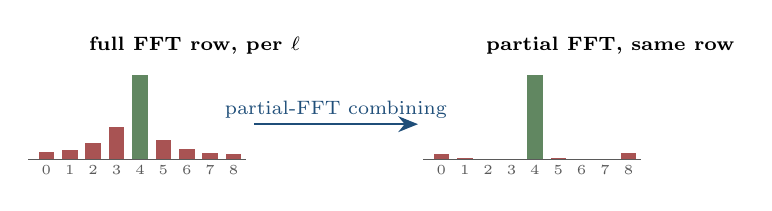
\begin{tikzpicture}[x=0.66cm,y=0.74cm]
  % left bars: full FFT
  \node[font=\scriptsize\bfseries] at (-4.0,1.95) {full FFT row, per $\ell$};
  \foreach \i/\h/\col in {0/0.12/accentred,1/0.16/accentred,2/0.27/accentred,3/0.55/accentred,4/1.45/accentgreen,5/0.32/accentred,6/0.18/accentred,7/0.10/accentred,8/0.09/accentred} {
    \fill[\col!75] (-7.0+\i*0.45,0) rectangle ++(0.30,\h);
    \node[font=\tiny,color=inkgray] at (-6.85+\i*0.45,-0.18) {\i};
  }
  \draw[inkgray] (-7.2,0) -- (-3.0,0);

  % right bars: partial FFT
  \node[font=\scriptsize\bfseries] at (4.0,1.95) {partial FFT, same row};
  \foreach \i/\h/\col in {0/0.08/accentred,1/0.02/accentred,2/0.01/accentred,3/0.01/accentred,4/1.45/accentgreen,5/0.015/accentred,6/0.01/accentred,7/0.01/accentred,8/0.10/accentred} {
    \fill[\col!75] (0.6+\i*0.45,0) rectangle ++(0.30,\h);
    \node[font=\tiny,color=inkgray] at (0.75+\i*0.45,-0.18) {\i};
  }
  \draw[inkgray] (0.4,0) -- (4.6,0);

  % arrow between
  \draw[flowarr,color=accentblue,line width=0.9pt] (-2.85,0.6) -- (0.30,0.6);
  \node[font=\scriptsize\color{accentblue}] at (-1.28,0.85) {partial-FFT combining};
\end{tikzpicture}
\end{center}

\bottomnote{Same diagonal height; the off-diagonal bars (the leaks) are much smaller after combining.}
\end{frame}

% =====================================================================
% 4f. RPC and JUNA choose the weights
% =====================================================================
\begin{frame}{4f. Who chooses the partial-FFT weights?}
\stagefourhdr{6}{RPC uses pilots; JUNA adds LDPC checks as another anchor}
\small
\begin{columns}[T,onlytextwidth]
  \begin{column}{0.48\textwidth}
    Partial FFT gives the receiver a branch vector:
    \[
      \mathbf z_k=[z_{0,k},z_{1,k},\ldots,z_{M-1,k}]\T.
    \]
    The receiver still needs carrier-specific weights:
    \[
      \widetilde y_k=\mathbf w_k^H\mathbf z_k.
    \]
    \vspace{-0.05cm}
    The weights should satisfy the two jobs we just saw:
    \[
      \mathbf w_k^H\mathbf c_{k,k}\approx 1,
      \qquad
      \mathbf w_k^H\mathbf c_{k,\ell}\approx 0
      \quad(\ell\ne k).
    \]
  \end{column}
  \begin{column}{0.50\textwidth}
    \begin{center}
    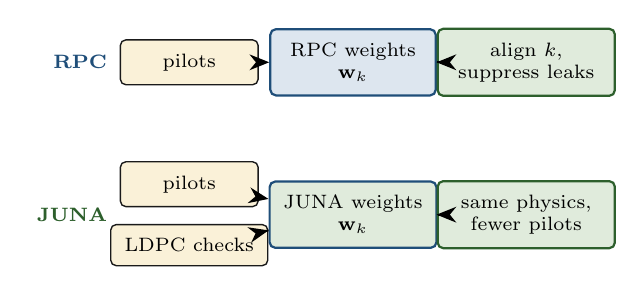
\begin{tikzpicture}[x=0.80cm,y=0.86cm,>=Latex]
      % RPC row
      \node[font=\scriptsize\bfseries\color{accentblue},anchor=east] at (-2.05,1.25) {RPC};
      \node[notecard,minimum width=1.75cm,font=\scriptsize] (pilots1) at (-0.90,1.25) {pilots};
      \node[bluecard,minimum width=2.10cm,font=\scriptsize,align=center] (rpcw) at (1.70,1.25)
        {RPC weights\\ $\mathbf w_k$};
      \node[greencard,minimum width=2.25cm,font=\scriptsize,align=center] (out1) at (4.45,1.25)
        {align $k$,\\ suppress leaks};
      \draw[flowarr] (pilots1) -- (rpcw);
      \draw[flowarr] (rpcw) -- (out1);
      % JUNA row
      \node[font=\scriptsize\bfseries\color{accentgreen},anchor=east] at (-2.05,-1.00) {JUNA};
      \node[notecard,minimum width=1.75cm,font=\scriptsize] (pilots2) at (-0.90,-0.55) {pilots};
      \node[notecard,minimum width=1.75cm,font=\scriptsize] (ldpc) at (-0.90,-1.45) {LDPC checks};
      \node[bluecard,minimum width=2.10cm,fill=grnbg,font=\scriptsize,align=center] (junaw) at (1.70,-1.00)
        {JUNA weights\\ $\mathbf w_k$};
      \node[greencard,minimum width=2.25cm,font=\scriptsize,align=center] (out2) at (4.45,-1.00)
        {same physics,\\ fewer pilots};
      \draw[flowarr] (pilots2) -- (junaw);
      \draw[flowarr] (ldpc) -- (junaw);
      \draw[flowarr] (junaw) -- (out2);
    \end{tikzpicture}
    \end{center}
  \end{column}
\end{columns}
\bottomnote{Partial FFT is the front-end physics trick. RPC and JUNA differ in how they learn reliable weights under limited pilots.}
\end{frame}

% =====================================================================
% Final mental model
% =====================================================================
\begin{frame}{Putting it all together}
\stepbadgehdr{$\bigstar$}{the chronological story in one line}
\footnotesize
\begin{center}
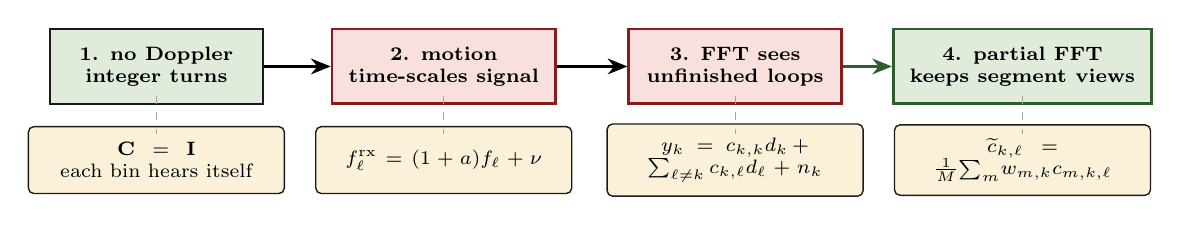
\begin{tikzpicture}[x=1.0cm,y=0.82cm,>=Latex]
  \node[flowbox,minimum width=2.7cm,minimum height=0.95cm,font=\scriptsize\bfseries,fill=grnbg] (a) at (-5.5,0.95)
    {1. no Doppler\\integer turns};
  \node[issue,  minimum width=2.7cm,minimum height=0.95cm,font=\scriptsize\bfseries] (b) at (-1.85,0.95)
    {2. motion\\time-scales signal};
  \node[issue,  minimum width=2.7cm,minimum height=0.95cm,font=\scriptsize\bfseries] (c) at (1.85,0.95)
    {3. FFT sees\\unfinished loops};
  \node[method, minimum width=2.7cm,minimum height=0.95cm,font=\scriptsize\bfseries] (d) at (5.5,0.95)
    {4. partial FFT\\keeps segment views};
  \draw[flowarr,line width=1pt] (a) -- (b);
  \draw[flowarr,line width=1pt] (b) -- (c);
  \draw[flowarr,line width=1pt,color=accentgreen] (c) -- (d);

  \node[notecard,text width=2.9cm,minimum height=0.85cm,font=\scriptsize] at (-5.5,-0.50)
    {$\mathbf C=\mathbf I$\\\scriptsize each bin hears itself};
  \node[notecard,text width=2.9cm,minimum height=0.85cm,font=\scriptsize] at (-1.85,-0.50)
    {$f_\ell^{\rx}=(1+a)f_\ell+\nu$};
  \node[notecard,text width=2.9cm,minimum height=0.85cm,font=\scriptsize] at (1.85,-0.50)
    {$y_k = c_{k,k}d_k\,+$\\$\sum_{\ell\ne k}c_{k,\ell}d_\ell+n_k$};
  \node[notecard,text width=2.9cm,minimum height=0.85cm,font=\scriptsize] at (5.5,-0.50)
    {$\widetilde c_{k,\ell}=\tfrac{1}{M}\!\sum_m\! w_{m,k}c_{m,k,\ell}$};

  % thin connecting strokes from each row box to its formula card
  \foreach \xpos in {-5.5,-1.85,1.85,5.5} {
    \draw[inkgray!55,line width=0.4pt,dashed] (\xpos,0.50) -- (\xpos,-0.10);
  }
\end{tikzpicture}
\end{center}

\vspace{0.08cm}
\begin{center}
\begin{tikzpicture}
  \node[draw=accentgreen,fill=grnbg,line width=0.9pt,rounded corners=4pt,
        text width=13.6cm,inner sep=7pt,align=center,font=\scriptsize] {%
    \textbf{One-sentence takeaway.}\,\,
    Motion turns each carrier's closed loop into an unfinished spiral; partial FFT keeps multiple short-window views so the receiver can rotate the desired arrow back into alignment while the leak arrows scramble.
  };
\end{tikzpicture}
\end{center}

\vspace{0.08cm}
{\scriptsize
\begin{columns}[T,onlytextwidth]
  \begin{column}{0.49\textwidth}
    \textbf{You can now picture}
    \begin{itemize}\setlength{\itemsep}{-0.10em}
      \item a carrier as a clock making $\ell$ turns per symbol,
      \item Doppler as a small fractional spin that ruins closure,
      \item ICI as the leftover arrow from the unfinished loop.
    \end{itemize}
  \end{column}
  \begin{column}{0.49\textwidth}
    \textbf{Where this leads (JUNA / RPC)}
    \begin{itemize}\setlength{\itemsep}{-0.10em}
      \item RPC trains the weights from pilots alone,
      \item JUNA adds LDPC confidence as a second anchor,
      \item same physics, fewer pilots needed.
    \end{itemize}
  \end{column}
\end{columns}}

\end{frame}

\end{document}
